\documentclass[]{article}

%% Minted work-around
\usepackage[section, outputdir=build]{minted}
% Input and output text encoding
\usepackage[T1]{fontenc}
\usepackage[utf8]{inputenc}

%%
%% Handy stuff
%%
\usepackage[english]{babel}
\usepackage[table,xcdraw]{xcolor}

% Set font size relative to the current font size
\usepackage{relsize}
% Space in custom commands
\usepackage{xspace}
% String manipulation
\usepackage{xstring}
% Typographical perfection
\usepackage{microtype}

% Text Companion fonts
\usepackage{textcomp}
% Font containing web-related icons
\usepackage{fontawesome}
% Format menu sequences, paths and keystrokes from lists
\usepackage[os=win]{menukeys}

%%
%% Graphics
%%
\usepackage{tikz}
\usepackage{graphicx}
\usepackage{rotating}
\usepackage{floatpag}
\usepackage{changepage}
\usepackage{subfig}
\usepackage[percent]{overpic}
\usepackage{caption}
\captionsetup{
    tableposition=top,
    figureposition=bottom,
    font=small,
    format=hang, 
    labelfont={sf,bf}
}

% Simple colour palette
\definecolor{darkgrey}{HTML}{787878}
\definecolor{backcolor}{HTML}{f7f7f7}
\definecolor{accent}{HTML}{c80900}
\definecolor{lightblue}{HTML}{00b6ff}

%%
%% Layout
%%

\usepackage{lastpage}
\usepackage{fancyhdr}
\usepackage{geometry}

% Hyphenation for letterspacing, underlining, and more
\usepackage{soul}

% Higher quality tables
\usepackage{booktabs}
% Tabulars with adjustable-width columns
\usepackage{tabularx}
% Coloured rows, columns, cells
\usepackage{colortbl}
% Control layout of itemize, enumerate, description
\usepackage[inline]{enumitem}

%%
%% Code listing
%%
\setminted[]{
  frame=lines,
  linenos=false,
  framesep=2mm,
  baselinestretch=1.2,
  bgcolor=backcolor,
  fontsize=\scriptsize,
  samepage=false,
  obeytabs=true,
  tabsize=2
}

\usepackage{algpseudocode}

%%
%% Physics, Math
%%

\usepackage{siunitx}
\sisetup{
  detect-all=true,
  input-digits = 0123456789\pi,
  per-mode = symbol,
  complex-root-position = before-number,
  output-complex-root = j,
  separate-uncertainty=true,
}

\usepackage{mathtools}
\allowdisplaybreaks[1]
\usepackage{amsfonts}
\usepackage{amsthm}

% Complex numbers for electrotechnics
\usepackage{steinmetz}
% Extended integrals
\usepackage{esint}
% Vector support
\usepackage[e]{esvect}
% Easy o&p derivatives
\usepackage{derivative} 
% Indicator function \mathbbm{1}
\usepackage{bbm}
% Left superscripts
\usepackage{tensor}


%%
%% User data
%%

\newcommand{\Id}{01NWMOQ \xspace}
\newcommand{\Course}{Electronics for Embedded Systems}
\newcommand{\Date}{\today}
\newcommand{\Title}{Experimental Project}
\newcommand{\Authors}{Fabio Scatozza (315216)}

%%
%% Page data
%%

\geometry{
  a4paper,
  top=2.54cm,bottom=2.54cm,left=2.54cm,right=2.54cm,
  headheight=25pt,
  heightrounded,includeheadfoot}
\pagestyle{fancyplain}
\lhead{\Id - \Course \\ \Title}
\rhead{}
\cfoot{}
\rfoot{\thepage/\pageref{LastPage}}
\renewcommand{\footrulewidth}{0.4pt}

%%
%% Hyperref & biblio
%%
\usepackage[autostyle,italian=guillemets]{csquotes}
\usepackage[style=numeric-comp,backend=biber]{biblatex}
\addbibresource{ref.bib}
\nocite{*}

\usepackage[nolist]{acronym}
\usepackage{hyperref, cleveref}
\hypersetup{
  colorlinks=false,
  pdfstartpage=1, pdfstartview=FitV, pdfborder={0 0 0},
  breaklinks=true, pageanchor=true,
  pdftitle={(\Id) \Title},
  pdfauthor={},
  pdfcreator={pdfLaTeX},
  pdfproducer={LaTeX with hyperref}
}

\title{\textbf{\Course}\\\Title}
\author{\Authors}
\date{\Date}

%%
%% Custom macros
%%

%%
%% Common
%%

% ** Symbols
\renewcommand{\epsilon}{\varepsilon}
\newcommand{\one}{\scalebox{1.2}{$\mathbbm{1}$}}

% ** Complex numbers
\let\Re\real
\DeclareMathOperator{\Re}{Re}
\let\Im\imaginary
\DeclareMathOperator{\Im}{Im}

% ** Fields
\newcommand{\field}[1]{\ensuremath{\mathbb{#1}}}
\newcommand{\C}{\field{C}}
\newcommand{\R}{\field{R}}
\newcommand{\N}{\field{N}}

% ** Automatic sizing delimiters
\DeclarePairedDelimiter{\pqty}{\lparen}{\rparen}
\DeclarePairedDelimiter{\bqty}{\lbrack}{\rbrack}
\DeclarePairedDelimiter{\Bqty}{\lbrace}{\rbrace}
\DeclarePairedDelimiter{\abs}{\lvert}{\rvert}
\DeclarePairedDelimiter{\avg}{\langle}{\rangle}
\DeclarePairedDelimiter{\eval}{.}{\rvert} % to be used only as \eval*
\DeclarePairedDelimiter{\peval}{\lparen}{\rvert}

% ** Vector notation
\newcommand{\va}[1]{\vv{\mathbf{#1}}} % vector arrow
\newcommand{\vu}[1]{\hat{\mathbf{#1}}} % unit vector
\newcommand{\vuG}[1]{\boldsymbol{\hat{#1}}} % unit vector Greek support

% ** Differential operators
\DeclareMathOperator{\grad}{\nabla}
\let\div\relax
\DeclareMathOperator{\div}{\nabla\cdot}
\DeclareMathOperator{\curl}{\nabla\times}
\DeclareMathOperator{\lapl}{\nabla^2}

% ** Derivatives
\newcommand{\oodif}[1]{\odif*[order=2]{#1}}
\newcommand{\ppdv}[1]{\pdv*[order=2]{}{#1}}

% ** Unit of measurement
\DeclareSIUnit{\rpm}{rpm}
\DeclareSIUnit{\ppm}{ppm}


\begin{document}
\begin{acronym}
    \acro{hps}[HPS]{Hard Processor System}
    \acro{mtbf}[MTBF]{Mean Time Between Failures}
\end{acronym}
\maketitle
\tableofcontents
\vfill
\printbibliography
\clearpage

\section{Introduction}

The \emph{Electronics for Embedded Systems} course explores the analog and digital aspects of embedded system design, focusing on the key components of their typical architecture. While sensor and actuator specifics are addressed in other courses, this course emphasizes the interface between the analog and digital domains, particularly A/D and D/A conversion, as well as the power electronics of actuator drivers and power supply devices. In the digital domain, the course spans software implementations running on microprocessors to hardware synthesized on programmable devices, with an emphasis on the underlying technology enabling computation, communication, and storage. Specifically, this involves analyzing the theory of programmable logic devices, microprocessor embedded peripherals, wired communication protocols, and memories.

In this context, the document presents a small-scale project aimed at addressing the key topics of the course, demonstrating competency aligned with the expected learning outcomes.

\section{Theory of Operation}\label{sec:theory_operation}

\begin{figure}
    \centering
    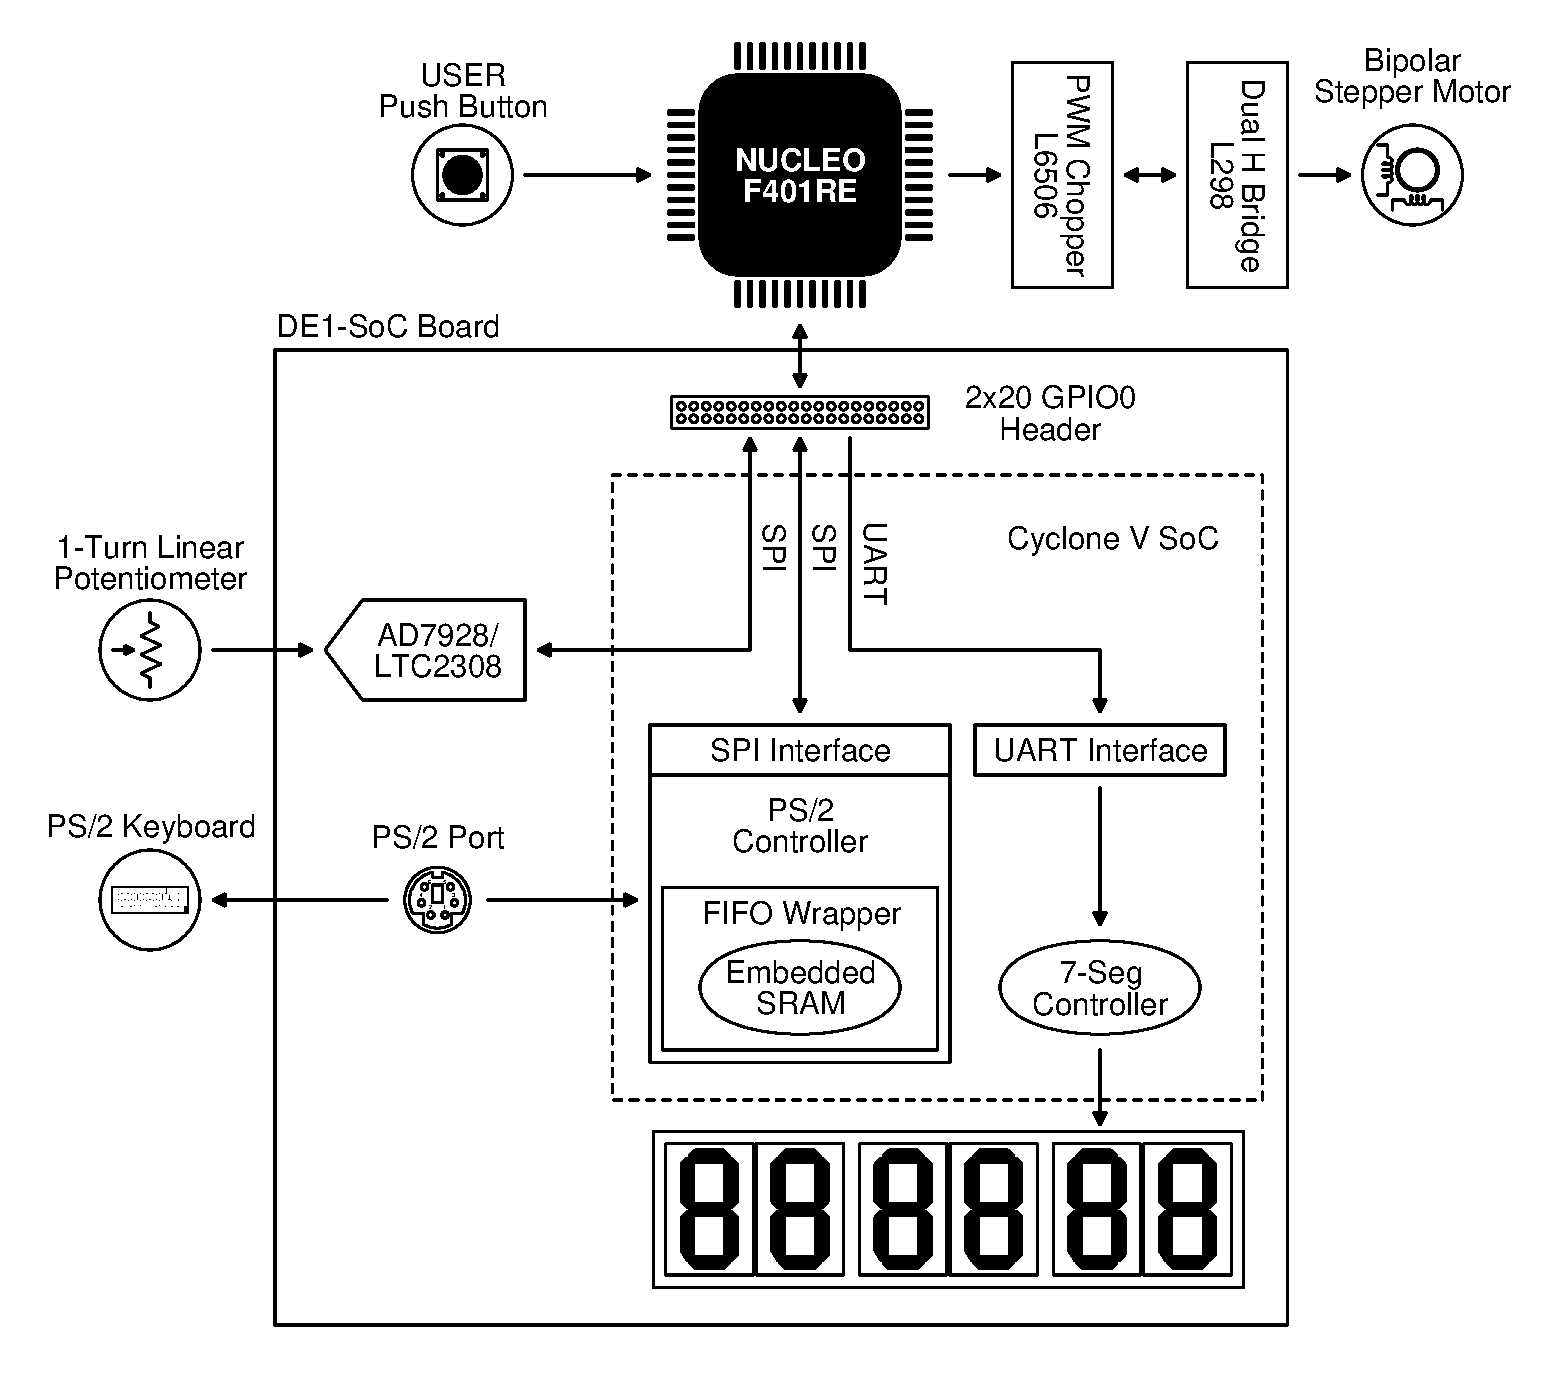
\includegraphics[width=\linewidth]{../gfx/system_diagram.eps}
    \caption{System block diagram}
    \label{fig:sys}
\end{figure}

The system implements an interface to program the movement pattern for a bipolar stepper motor and execute it on demand. The pattern is committed to non-volatile storage and consists of a sequence of data points, each representing a circular motion segment defined by angular velocity and displacement. During execution, the data points are retrieved in a circular fashion from memory, and are converted into motor-driving stimuli.
Referring to the system block diagram in~\cref{fig:sys}, the interface is operated as follows.
\begin{itemize}
    \item The movement pattern is cleared by pressing and holding the user push button for at least \qty{1}{\s}. Successful clearing is acknowledged by displaying \emph{CLEAr} on the 7-segment displays.
    
    \item Data points are entered using the linear potentiometer and the PS/2 keyboard. The potentiometer sets the angular velocity in the range from \qtyrange{2.5}{400}{\rpm}, while the angular displacement is specified in degrees with the keyboard, according to the following regex pattern.
    \begin{center}
    \begin{BVerbatim}
    [+-]?[0-9]{1,3}(\.[0-9])?
    \end{BVerbatim}
    \end{center}
    The sign defaults to \verb|+| if omitted, which corresponds to a counterclockwise rotation. The integer part is specified with up to three digits, whereas the fractional part is optionally specified with one digit.
    Due to the inherently discrete nature of the stepper motor rotation and accounting for the two-phases-on driving method, the target angular displacement is rounded to the nearest value that minimizes error.

    When the data point entry begins, triggered by pressing some keys, the 7-segment displays change to \emph{InPUt}. The operation is terminated by pressing the return \keys{\return} or \keys{\enter} keys, upon which data is validated, and the potentiometer output is converted. The outcome is notified as follows: \emph{Err-2 bAd PAttErn}, if the parsing of the keyboard input failed; \emph{Err-3 FuLL}, if the maximum number of data points have already been entered. Otherwise, if no error has occurred, the data point is displayed in the format below, where the data point number starts at zero, the angular velocity is expressed in revolutions per minute, and the angular displacement in degrees.
    \begin{center}
    \begin{BVerbatim}
    [<data point number>] <angular velocity> <angular displacement>
    \end{BVerbatim}
    \end{center}

    \item The execution of a valid movement pattern, that is, one containing at least one data point, begins by pressing the user push button. An empty pattern results in the display of \emph{Err-1 no dAtA}, while a valid pattern displays \emph{PLAy}. The execution continues until the push button is pressed again, after which the displays revert to printing \emph{IdLE}.
\end{itemize}

\section{System Design}\label{sec:sys_design}

\begin{figure}
    \centering
    \subfloat[][Quartus Prime RTL view\label{fig:fpga_rtl}]{
        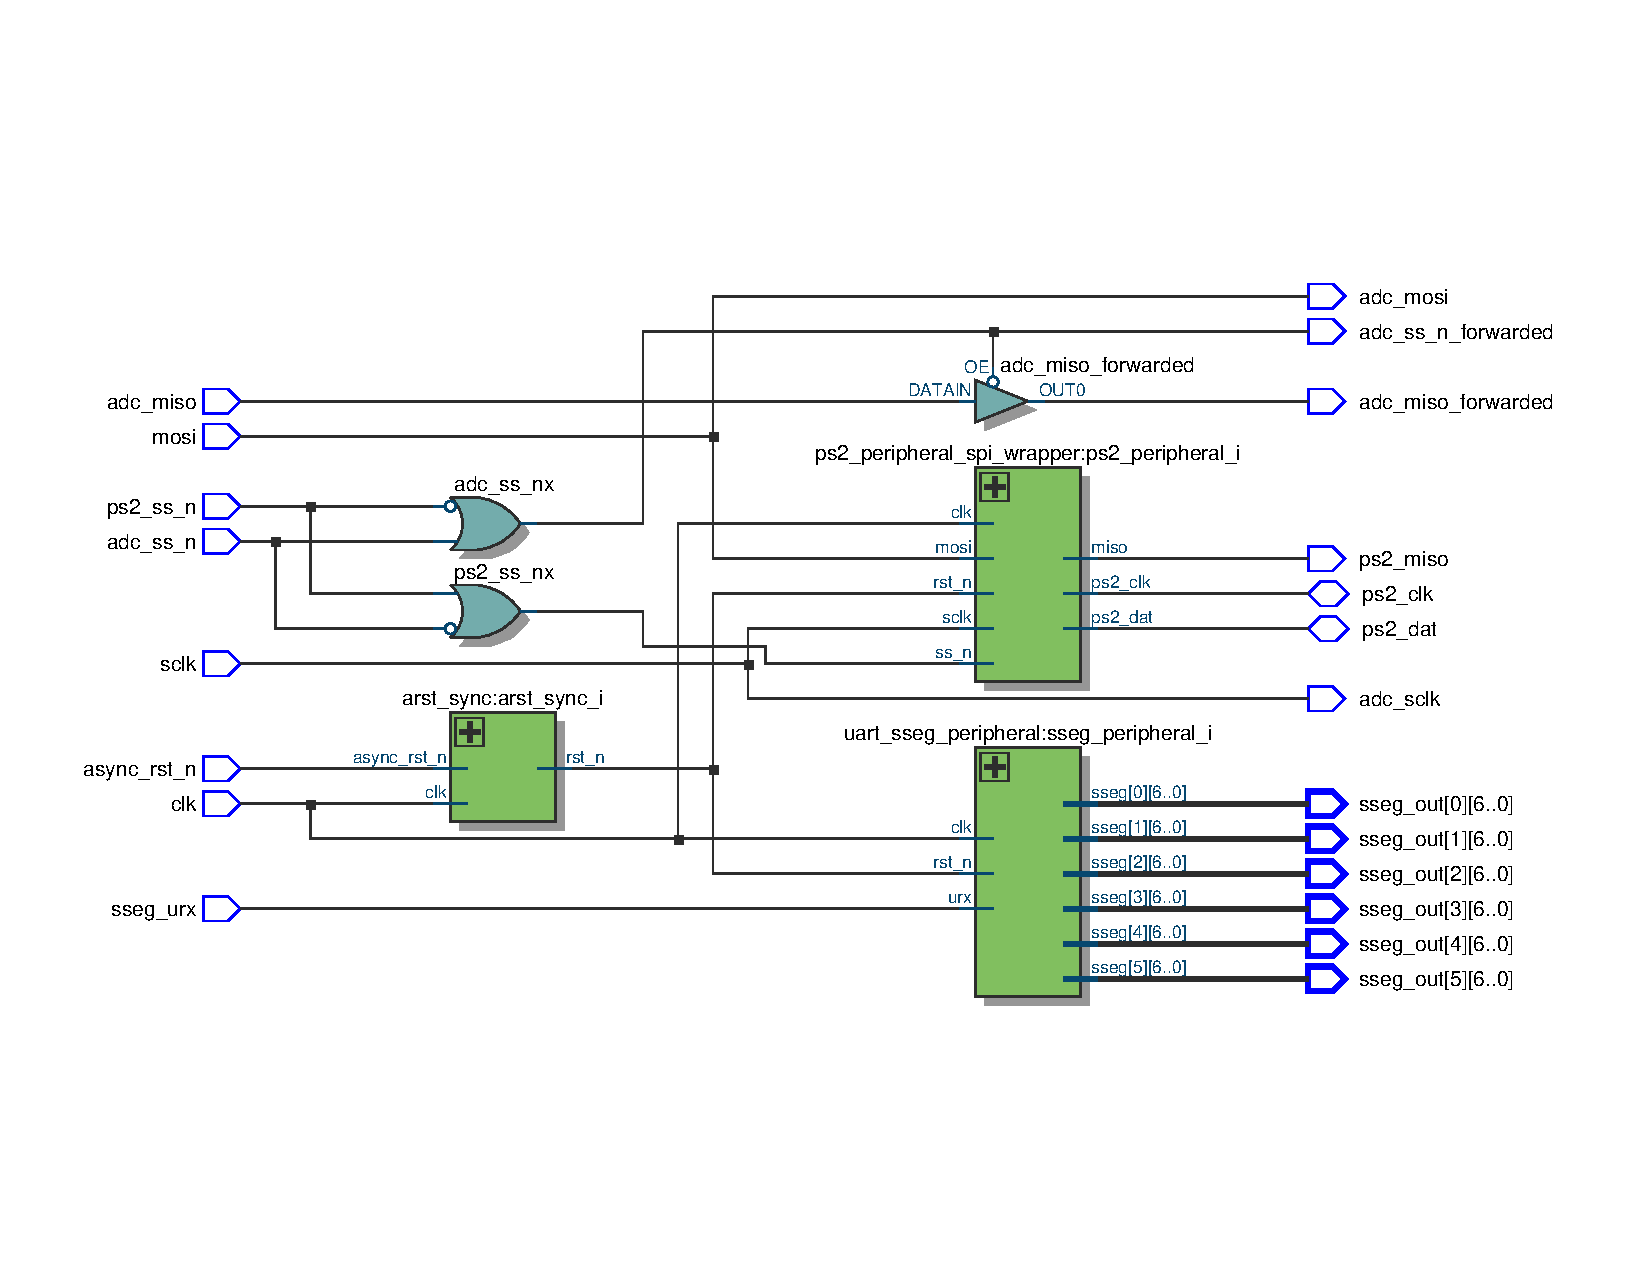
\includegraphics[width=\linewidth]{../gfx/RTLview.pdf}
    }\\
    \subfloat[][Signals mapped to the 2x20 header for interfacing with the MCU\label{fig:fpga_port}]{
        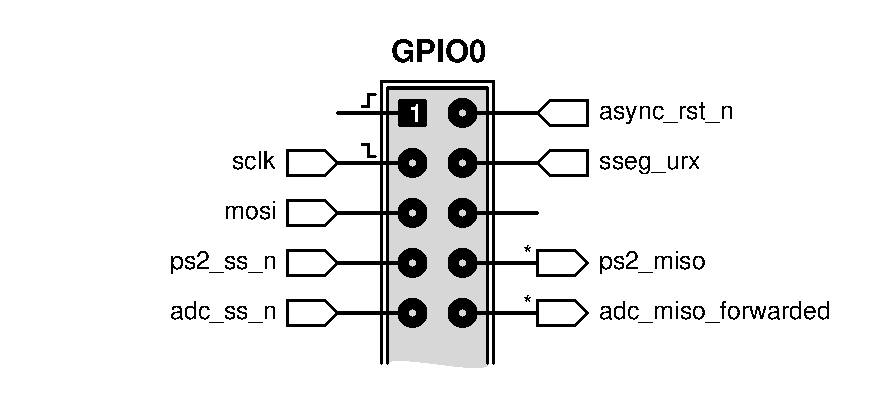
\includegraphics[scale=.65]{../gfx/GPIOHeader.eps}
    }
    \caption{DE1-SoC board subsystems}
    \label{fig:de1_soc}
\end{figure}

\begin{figure}
    \centering
    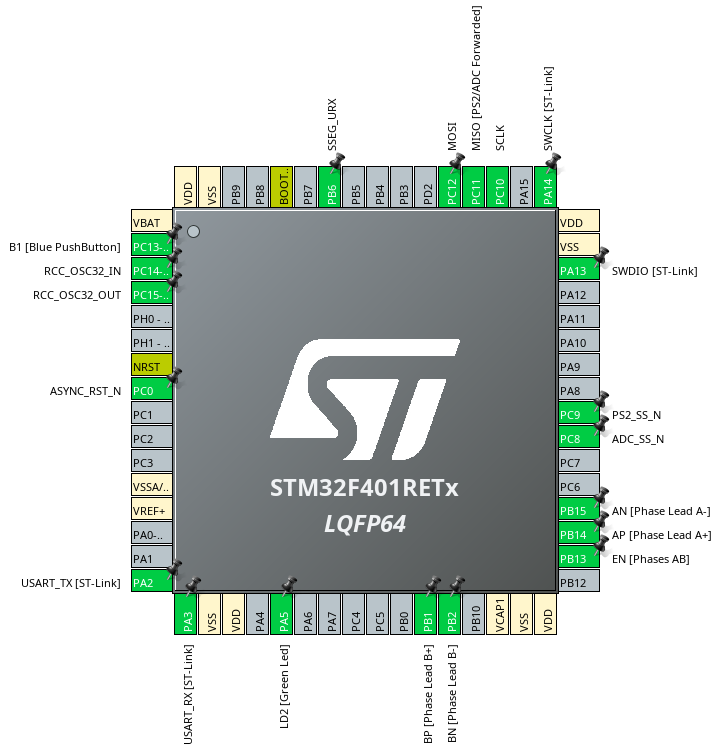
\includegraphics[width=.65\linewidth]{../gfx/mcu_pinout.png}
    \caption{Microcontroller pinout (generated by STM32CubeMX~\cite{cubemx}).}
    \label{fig:mcu_pins}
\end{figure}

\begin{figure}
    \centering
    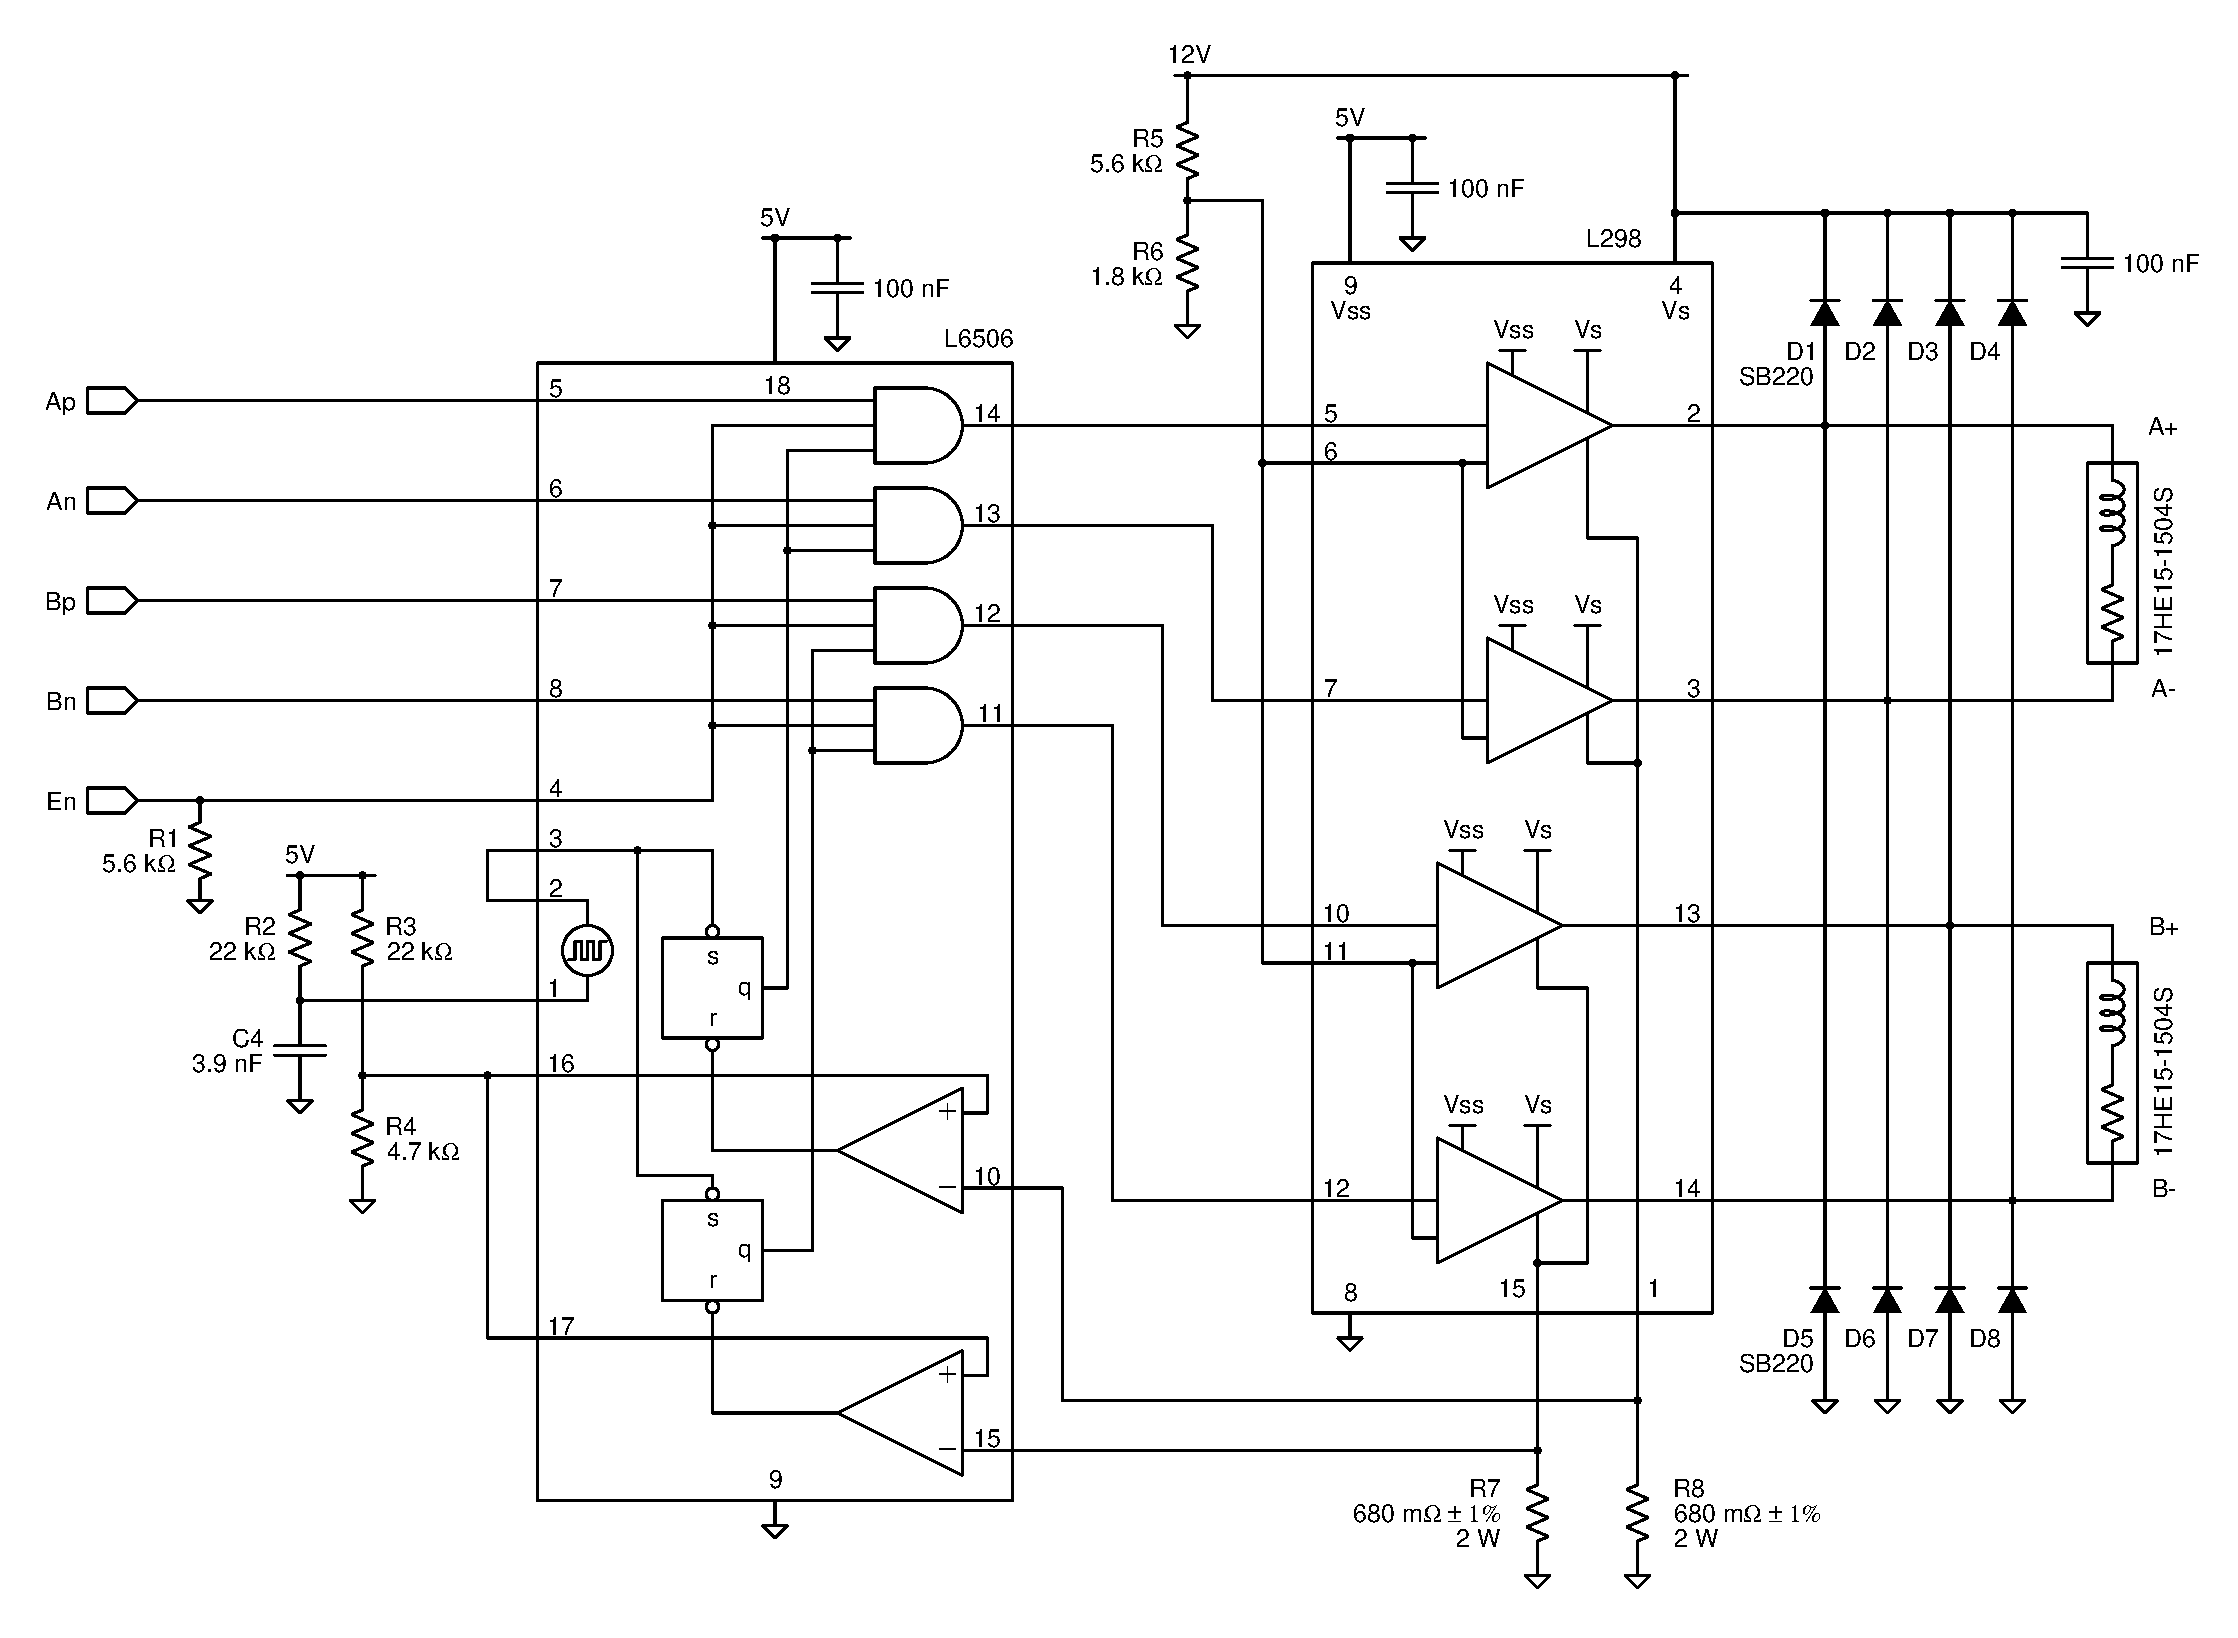
\includegraphics[width=.8\linewidth]{../gfx/motor_board.eps}
    \caption{Drive circuit for the bipolar stepper motor. The L6506 senses and controls the current in the motor windings, which are energized with the dual full-bridge driver L298.}
    \label{fig:motor_bd}
\end{figure}

The system is devised to target the hardware available on the design platform employed for the laboratory activities of the course, the DE1-SoC development kit by Terasic~\cite{de1soc}. The platform is built around Altera's Cyclone V SE SoC device~\cite{cyclone}, which integrates an ARM-based \ac{hps} tied to the FPGA fabric with an on-chip interconnect.
Potentially, this kit alone allows to experiment with digital processing in the form of software running on a hard or soft microprocessor to program hard and soft peripherals, as well as by synthesizing dedicated hardware. Despite this flexibility, the processor system is implemented with an external microcontroller development board, the NUCLEO-F401RE by STMicroelectronics~\cite{nucleo}, thus creating the opportunity to investigate communication protocols for wired interconnections.
As illustrated in the block diagram of~\cref{fig:sys}, the system comprises:
\begin{itemize}
    \item Input devices.
    \begin{itemize}
        \item The user and reset push buttons are part of the microcontroller development board.
        \item The linear potentiometer is wired to the ADC available on the DE1-SoC board, through the dedicated 2x5 header. This is discussed in~\cref{subsec:adc}.
        \item The PS/2 keyboard is attached to the corresponding port on the DE1-SoC board, through the fitted 6-pin mini-DIN connector.
    \end{itemize}
    
    \item Peripherals and glue logic implemented on the FPGA target, as more accurately shown in~\cref{fig:fpga_rtl}.
    The interface to the microcontroller consists of the signals mapped to the 2x20 expansion header GPIO0, as depicted in~\cref{fig:fpga_port}.
    \begin{itemize}
        \item The SPI-compatible port of the converter is routed through the FPGA fabric, up to the GPIO0 header.
        \item An asynchronous reset signal driven by the microcontroller is brought into the FPGA \qty{50}{\MHz} clock domain, to be used as a synchronously deasserted system-wide reset.
        \item The PS/2 peripheral implements the PS/2 protocol to communicate with the keyboard device, while it exposes an SPI port to the microcontroller. The design of the module is presented in~\cref{subsec:ps2}.
        \item The display peripheral drives the 7-segment displays available on the DE1-SoC board with the character stream received from the microcontroller via UART. This is discussed in~\cref{subsec:sseg}.
    \end{itemize}
    The slave select inputs are internally pulled up, to ensure an inactive level while the microcontroller resets.

    The blocks are modeled in SystemVerilog and are functionally simulated with testbenches that make use of the verification subset of the language. The approach to verification is directed testing, with non-constrained randomized stimuli. As a result, the testbenches can be run with the freeware edition of Questa Intel Starter FPGA Edition.
    The synthesis flow is carried out with the Quartus Prime Lite toolchain, using bash and Tcl automation scripts.

    \item Microcontroller and bipolar stepper motor drive circuit, as illustrated in greater details in~\cref{fig:mcu_pins,fig:motor_bd}.
    The microcontroller development board, the L6506 controller~\cite{l6506}, and the logic section of the L298 driver~\cite{l298}, are powered at \qty{5}{\V} from the DE1-SoC board; the microcontroller power supply is further regulated down to \qty{3.3}{\V}.
    \begin{itemize}
        \item As the FPGA I/Os are configured in the \qty{3.3}{\V} LVTTL standard, the microcontroller directly interfaces to the signals on the 2x20 header GPIO0. Notably, the PS/2 and ADC MISO signals are wired as a shared line into the microcontroller, and the input is internally pulled down to ensure a well-defined logic level while neither slave is selected.

        Several peripherals are configured to achieve the desired functionality, most importantly:
        \begin{itemize}
            \item The GPIO, to detect push button presses, as well as for generating reset and enable signals for the FPGA subsystem and its peripherals.
            \item The SPI3, USART1, and DMA2 to communicate with the peripherals synthesized in the FPGA.
            \item The TIM1 and DMA2, to generate two pairs of complementary square waveforms, with one pair in quadrature to the other, to drive the bipolar stepper motor.
        \end{itemize}
        Furthermore, one sector of the embedded NOR flash memory is used as a non-volatile circular buffer to store the motor movement pattern, and play it on demand. The architecture of the firmware is further explained in~\cref{sec:sw_design}.
        
        \item The L6506 inputs accept \qty{5}{\V} TTL levels, with $V_\text{IL} = \qty{0.8}{\V}$ and $V_\text{IH} = \qty{2}{\V}$. Consequently, the microcontroller can reliably drive them, without requiring any additional translation logic. During reset, the enable signal is pulled down with an external resistor.

        \item The L298 is permanently enabled. The datasheet prescribes that the enable signals of the H-bridges are to be driven low before turning on or off the power stage, which is achieved by means of the resistive divider $(R_5,\,R_6)$. 
    \end{itemize}
    The design of the circuit, for the bipolar stepper motor 17HE15-1504S~\cite{stepp}, is discussed in~\cref{subsec:motor_bd}.
\end{itemize}

\subsection{Angular Velocity Acquisition}\label{subsec:adc}

Depending on the board revision, the ADC is either the AD7928~\cite{ad7928} or the LTC2308~\cite{ltc2308}, which feature \qty{12}{\bit} of resolution with a successive approximation topology, and an SPI-compatible serial interface. The analog input range changes slightly between the two devices: for the AD7928, the full range can be digitally selected equal to the external \qty{2.5}{\volt} nominal reference or double its value. For the LTC2308 instead, it is fixed to \qty{4.096}{\volt}. In either case, the 2x5 dedicated header only provides access to the eight input channels, to the ground, and to the \qty{5}{\volt} supply rail, thus preventing measurements in a ratiometric configuration.
    
Accordingly, for the AD7928, a \qty{10}{\kohm} linear potentiometer is wired between the \qty{5}{\volt} supply rail and ground, with the wiper node connected to a single-ended input channel. The \qty{500}{\uA} nominal current through the voltage divider makes the \qty{1}{\uA} leakage current negligible.
In the worst case scenario for the sample and hold circuitry, the wiper of the potentiometer sits at halfway position, such that the output resistance of the thevenin equivalent $R_\text{s}$ is at its maximum value of \qty{2.5}{\kohm}. 
In this condition, with a typical hold capacitance $C_\text{h}$ of \qty{20}{\pF} and an equivalent input resistance $R_\text{in}$ of \qty{400}{\ohm}, a fully discharged hold capacitor charges up to the \qty{2.5}{\volt} input $V_\text{s}$ following
\[
    v_\text{h}\pqty*{t} = V_\text{s}\,\pqty*{1-e^{-t/\tau}}
    ,\qquad \text{with}\qquad \tau = \pqty*{R_\text{s}+R_\text{in}}\,C_\text{h}
\]
and the time required for this voltage to settle within half LSB of the final value is
\begin{equation}\label{eq:tset}
    t_\text{set} = \tau\,\ln\,\frac{V_\text{s}}{0.5 \,\text{LSB}}
\end{equation}
Hence, $t_\text{set} = \qty{482}{\ns}$ bounds the minimum acquisition time for achieving full resolution conversions.

Considering the narrower analog range of the LTC2308, the \qty{10}{\kohm} potentiometer is wired at the bottom of a voltage divider, with the resistor $R_1$ on the upper branch sized to limit the voltage drop on the potentiometer. Denoting with $V_\text{s}$ the supply voltage and with $V_\text{fr}$ the ADC full range, it must hold
\[
    V_\text{s}\,\frac{R_\text{pot}}{R_\text{pot} + R_1} \le V_\text{fr}
\]
Therefore, in the typical case for the supply and full range voltages, but considering a \qty{10}{\percent} uncertainty on the potentiometer resistance and a \qty{1}{\percent} uncertainty for $R_1$, it is required that
\[
    R_{1,\text{min}} \ge 
    R_{\text{pot},\text{max}}\,\pqty*{\frac{V_\text{s}}{V_\text{fr}}-1}
\]
which yields $R_1 \ge \qty{2.43}{\kohm}$. Accordingly, $R_1$ can be chosen in the E12 series with a nominal value of \qty{2.7}{\kohm}.
Finally, the observation on the minimum acquisition time for the AD7928 applies here too. Given the different configuration of the voltage divider, the output resistance is maximized when the wiper reaches a position where the total divider resistance is split in half, hence $R_\text{s}$ is \qty{3.18}{\kohm}. Considering the equivalent model of the analog input, with a typical hold capacitance $C_\text{h}$ of \qty{55}{\pF} and an equivalent input resistance $R_\text{in}$ of \qty{100}{\ohm}, \cref{eq:tset} yields $t_\text{set} = \qty{1.53}{\us}$.

The four signals of the ADC serial interface are routed through the FPGA fabric up to the 2x20 GPIO0 expansion header, where they connect to the microcontroller pins assigned to the SPI peripheral. The peripheral is configured as a full-duplex master, with software-controlled slave select signals.

\subsection{Angular Displacement Acquisition}\label{subsec:ps2}

\begin{figure}
    \centering
    \subfloat[][System receiving data. The device generates data while the clock is high.]{
        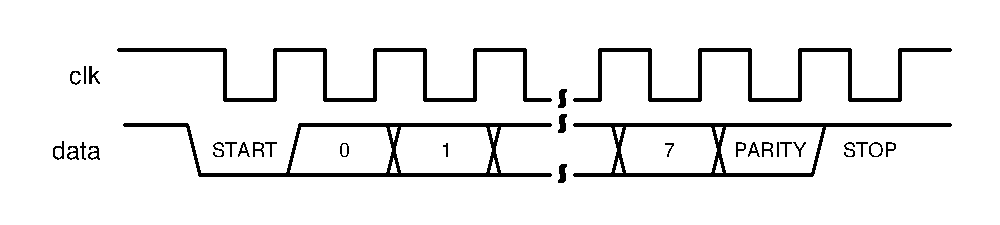
\includegraphics[width=.7\linewidth]{../gfx/ps2_timing_rx.eps}
    }\\
    \subfloat[][System sending data. The system generates data while the clock is low; following the parity bit, the device detects the stop bit and pulls the data line low while the clock is high (dashed portion of the waveform).]{
        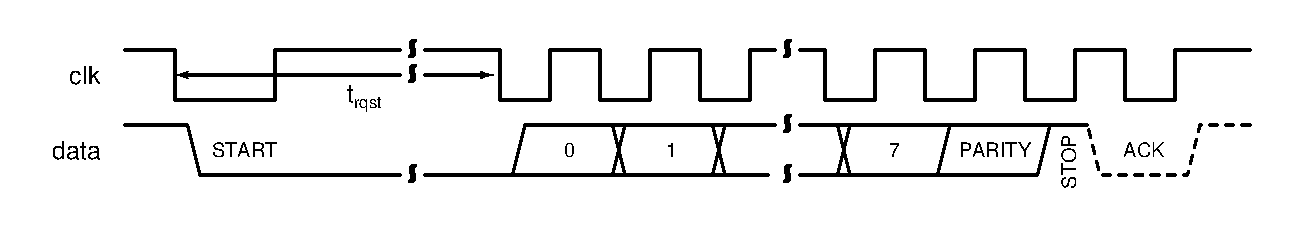
\includegraphics[width=.9\linewidth]{../gfx/ps2_timing_tx.eps}
    }
    \caption{PS/2 timing diagrams. The clock period ranges from \qtyrange{60}{100}{\micro\s}; the maximum request-to-send duration is \qty{15}{\milli\s}.}
    \label{fig:ps2_timing}
\end{figure}

The PS/2 protocol~\cite{ps2_controller,ps2_device} regulates the point-to-point bidirectional communication between the system and the keyboard device. It is a synchronous serial protocol in which data is time-multiplexed over a single data line, while a dedicated line carries the clock signal. Accordingly, the communication is half-duplex and both clock and data lines are shared with an open-drain architecture to avoid damage in case of conflicts.

The clock is always generated by the PS/2 device, but the system can pull the clock line low to inhibit the bus, potentially causing collisions that are used to abort ongoing transmissions in either direction. When the bus is not inhibited, two configurations are possible prior to a transmission: if the data line is also pulled high, the bus is in its idle state, which is the only one in which the device can initiate a transmission to the system. Alternatively, if the data line is held low by the system, the configuration signals the device that the system is ready to transmit data and awaiting clock generation.
The transmission is character-based and the frame comprises:
\begin{itemize}
    \item Start bit, always 0
    \item \qty{8}{\bit} character, transmitted LSB first
    \item Odd parity bit, either 0 or 1 such that the overall count of bits with value 1 in the character concatenated with the parity bit is odd
    \item Stop bit, always 1
\end{itemize}
The timing diagram for receiving and sending data are shown in~\cref{fig:ps2_timing}.

\subsubsection{PS/2 Peripheral}\label{ssubsec:ps22spi}

\begin{figure}
    \centering
    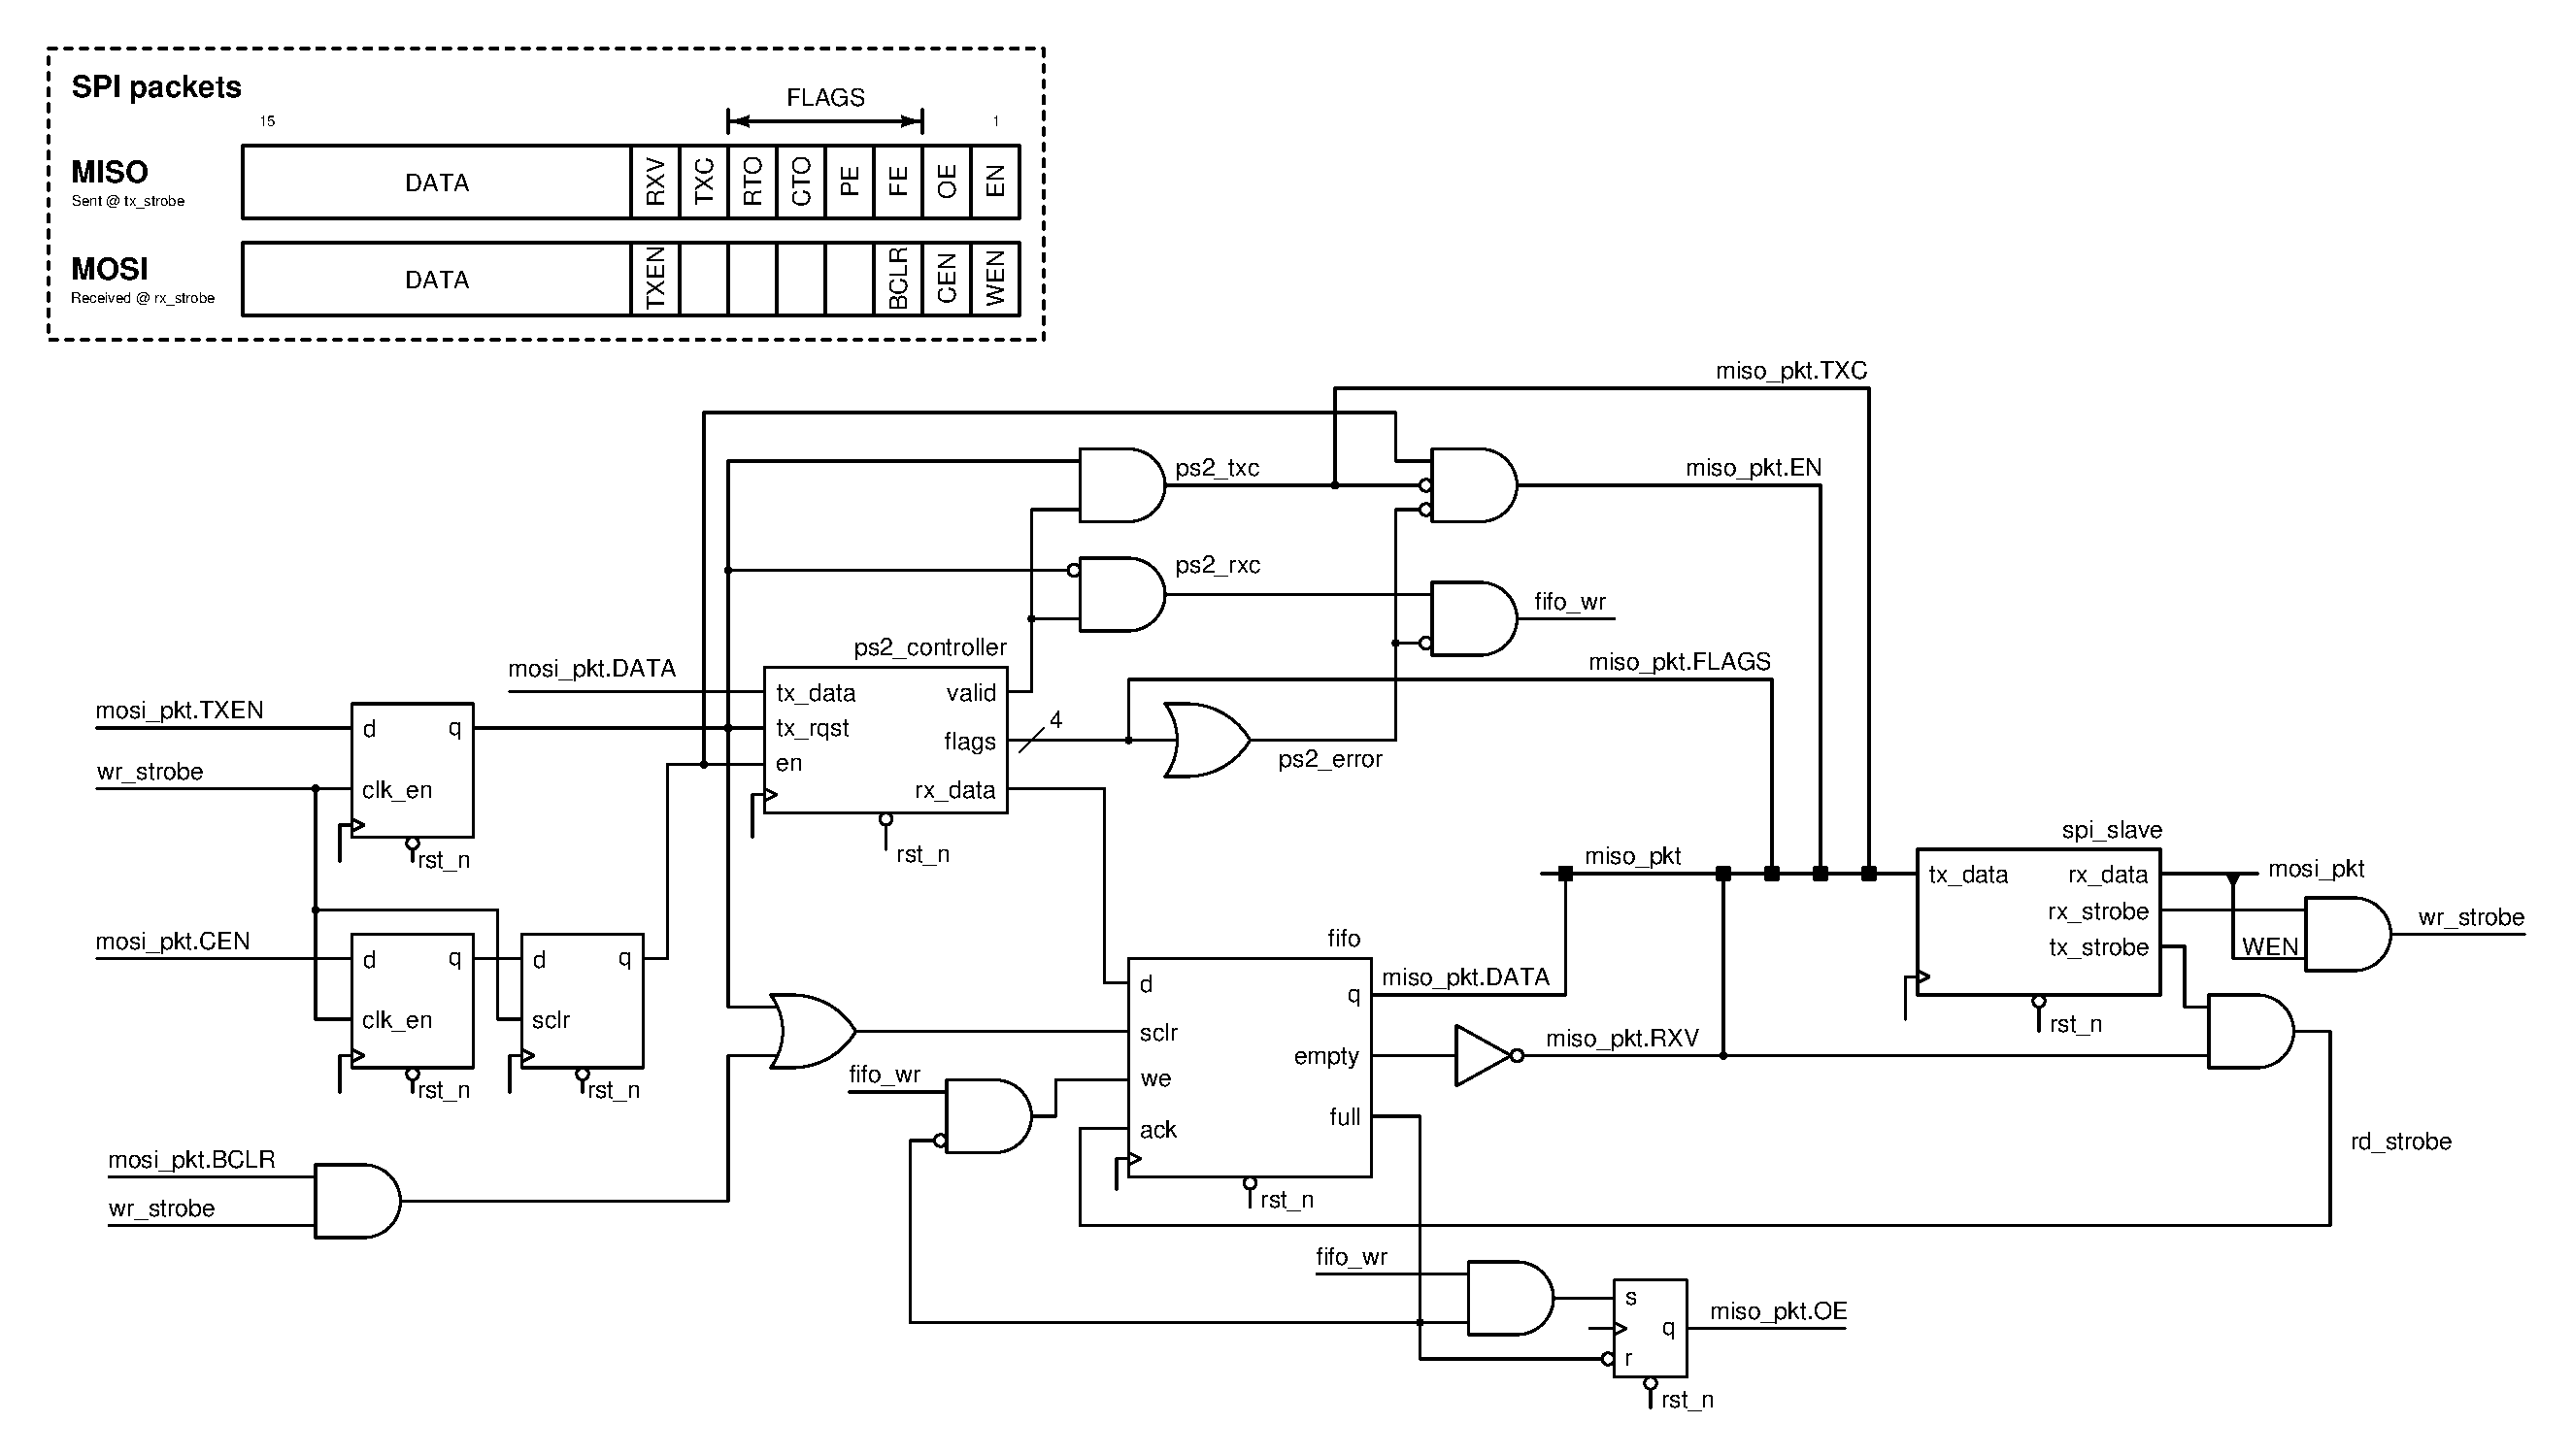
\includegraphics[width=\linewidth]{../gfx/ps2_peripheral_spi_wrapper.eps}
    \caption{SPI-compatible PS/2 controller peripheral design. The module implements the PS/2 protocol for exchanging data with a PS/2 device, exposing its control, status, and data registers through SPI. Data received from the device is buffered in an SRAM FIFO. The PS/2 and SPI buses are not shown.}
    \label{fig:ps2_peripheral}
\end{figure}

The PS/2 protocol is implemented by the custom peripheral shown in~\cref{fig:ps2_peripheral}, which enables data exchange with an external PS/2 device, under the control of an SPI-capable system. It includes three key modules: a PS/2 controller, a show-ahead single-clock FIFO, and an SPI slave controller. Additional glue logic implements the desired behavior for the control and status register bits that are exposed through SPI.

\begin{description}
    \item[PS/2 Controller] It implements the PS/2 protocol specifications and provides an higher-level simplified interface to the PS/2 device, as presented in~\cref{lst:ps2_controller}. It supports bidirectional communication and provides several reliability features. The data and clock lines are synchronized to the system clock domain with a flip-flop chain: the depth defaults to 2, which achieves a reasonable trade-off of latency and \ac{mtbf} due to metastable events. The controller detects:
    \begin{itemize}
        \item Frame errors. On reception, if the start or stop bit is missing at the expected time. On transmission, if the acknowledgment bit is similarly absent.
        \item Parity error, if the parity check fails during reception.
        \item Clock timeouts, if the falling edges of the clock are separated by more than \qty{150}{\micro\s} during either reception or transmission.
        \item Request timeouts. On transmission, if the device does not generate the clock within a \qty{15}{\milli\s} window after the system inhibits the PS/2 bus (see~\cref{fig:ps2_timing}).
    \end{itemize}
    
    The controller has been designed according to the ASM methodology, starting from a pseudocode description of the receive and transmit operations; the resulting ASM chart and data path are provided in~\cref{apx:ps2_controller}. In summary, the module operates as follows.
    \begin{itemize}
        \item On reset or while not enabled, the controller inhibits the bus by driving the clock line low.
        \item While enabled, with no pending transmission request, the controller monitors the bus for transmissions from the device. In case of successful reception, the valid signal pulses for one clock cycle and the received character appears on the data output. Conversely, in case of failure, the valid signal is held high while the flags signal the cause. While in this failure state, the PS/2 bus is inhibited; resuming normal operation requires a falling transition on the enable signal.
        \item While enabled, with no ongoing transmission to the device, the controller samples the data to be transmitted in the same clock cycle where the transmission request gets asserted. In case of successful transmission, the valid signal is held high until the request signal becomes inactive, and the bus is inhibited. Conversely, the failure behavior is the same as in reception.
    \end{itemize}

    \begin{listing}
    \begin{minted}{systemverilog}
    module ps2_controller #(
      parameter int unsigned SYNC_STAGES = 2,
      parameter real FCLK_HZ = 50e6,
      parameter int unsigned TIM_PSC = 249 // tim_fclk = fclk/(PSC+1) = 200 kHz, for 50 MHz clock
    ) (
      input var logic clk,
      input var logic rst_n,
      input var logic en,
    
      input var logic tx_rqst,
      input var logic [7:0] tx_data,
    
      output logic valid,
      output logic [7:0] rx_data,
      output ps2_pkg::flags_t flags,
    
      inout tri ps2_clk,
      inout tri ps2_dat
    );
    \end{minted}
    \caption{SystemVerilog interface of the PS/2 controller. The number of flip-flop synchronizing stages for the PS/2 lines is parameterized and defaults to 2. The timing thresholds are computed at compile-time, based on the specified clock frequency and prescaler value.}
    \label{lst:ps2_controller}
    \end{listing}

    \item[Show-Ahead Single-Clock FIFO] Data received from the PS/2 device is buffered in a synchronous FIFO structure with a show-ahead interface. Provided that the empty signal is inactive, this interface automatically outputs the first valid word, and asserting the read-acknowledge signal causes the FIFO to output the next valid word.

    The module is designed to infer embedded dual-port SRAM blocks if available, without depending on a specific read-during-write behavior. On reset, the read and write pointers are cleared, and the FIFO is empty. With the first write operation, the data is stored at the write pointer location, which is the same one being read: due to the read-during-write event, the SRAM may output the old data, thus the latency for the data to appear at the output is 2 clock cycles. Accordingly, the empty flag is cleared with the same latency. The full design is provided in~\cref{apx:fifo}.

    \item[SPI Slave Controller] It implements the SPI protocol in the slave role, with programmable frame length, clock polarity (CPOL) and clock phase (CPHA).

    To decrease clock oversampling requirements, the receive and transmit logic operate within the domain of the external SPI clock, generated by the master device; the slave select signal crosses into the system clock domain with a dual flip-flop synchronizer. While the slave is not selected, the data to be transmitted is sampled in the system clock domain up to one clock cycle before the transmit strobe signal pulses high, which marks the start of communication. At the end of the communication, when the slave is deselected, the received data is loaded onto the data output and becomes valid in the system clock cycle when the receive strobe signal pulses high.
    \Cref{apx:spi} contains the design of the module and the manual timing analyses.
    
\end{description}

The peripheral exposes its control, status, and data registers as packets exchanged through SPI, according to the format summarized in~\cref{fig:ps2_peripheral}. A detailed description of the packets format is provided below.
\begin{description}[style=nextline]
    \item[MOSI Packet]\hfill
    
        \begin{enumerate}[
            label=\emph{Bit \arabic*}, widest=s 15:8,
            left=\parindent, align=left,
            itemsep=2.5\itemsep,
            start=0
        ]
        \item \textbf{WEN}: Write Enable
        \begin{enumerate}[label=\arabic*:, start=0]
            \item The packet is discarded
            \item The packet is decoded
        \end{enumerate}
    
        \item \textbf{CEN}: Controller Enable
        \begin{enumerate}[label=\arabic*:, start=0]
            \item Disables the controller and inhibits the PS/2 bus (clock line low)
            \item Clears the flags (FE, PE, CTO, and RTO), and enables the controller in the operation mode set by TXEN.
            
            If the controller is already running (EN bit is set), the current operation is aborted. Aborting a receive operation while the PS/2 device is transmitting a character generates a communication error (FE, PE, or CTO set).
        \end{enumerate}
    
        \item \textbf{BCLR}: Buffer Clear
        \begin{enumerate}[label=\arabic*:, start=0]
            \item The receive FIFO buffer is not flushed
            \item The receive FIFO buffer is flushed. If both CEN and BCLR are set, the flush operation is performed prior to enabling the controller.
        \end{enumerate}
    
        \makeatletter
            \addtocounter{\@enumctr}{4}
        \makeatother
        
        \item \textbf{TXEN}: Transmitter Mode Enable
        
        This bit determines the operation mode.
        \begin{enumerate}[label=\arabic*:, start=0]
            \item The controller receives data from the PS/2 device.
            Incoming packets are stored in the FIFO buffer, whose state is represented by the RXV and OE status bits. When the FIFO is empty, the RXV bit is cleared and the DATA field is undefined. Otherwise, the RXV bit is set, and the DATA field is valid. If the FIFO buffer is full and new packets are received, the OE status bit is set. Each SPI transfer removes one element from the FIFO, which may also clear the OE bit. Alternatively, the OE bit is cleared by flushing the FIFO buffer when the BCLR control bit is set.
    
            \item The FIFO buffer is cleared, and the controller sends data to the PS/2 device. When the operation completes, the TXC bit is set, the flags are updated (FE, CTO, and RTO), the EN bit is cleared and the PS/2 bus is inhibited (clock line low).
        \end{enumerate}
    
        \item[\emph{Bits 15:8}] \textbf{DATA}: Transmit Data
        
        If TXEN is set, the data to be sent to the PS/2 device.
    \end{enumerate}
    
    \item[MISO Packet]\hfill
    
        \begin{enumerate}[
            label=\emph{Bit \arabic*}, widest=s 15:8,
            left=\parindent, align=left,
            itemsep=2.5\itemsep,
            start=0
        ]
            \item \textbf{EN}: Controller Enabled
            
            This bit is set by the master when enabling the controller and is cleared by the hardware in one of the following cases:
            \begin{itemize}
                \item The communication has failed and a flag is set (FE, PE, CTO, or RTO).
                \item The TXEN control bit enabled the controller in transmitter mode, and the transmission has terminated (TXC is set).
            \end{itemize}
            With the EN bit cleared, the PS/2 bus is inhibited (clock line low).
            
            \item \textbf{OE}: Overrun Error
            
            This bit is set by the hardware when the FIFO buffer is full and a new packet has been received and lost. It is automatically cleared when removing elements from the FIFO with SPI transfers, when flushing the buffer by setting the BCLR bit, or when the controller is enabled in transmitter mode.
            
            \item \textbf{FE}: Frame Error
    
            This bit is set by the hardware if the communication has failed in one of the following ways. While receiving data from the PS/2 device, either the START or STOP bits are not recognized at the expected time. While transmitting data, the ACK bit is not recognized at the expected time.
            
            Once the error is raised, the controller halts and inhibits the PS/2 bus (clock line low). Resuming normal operation requires enabling the controller again.
            
            \item \textbf{PE}: Parity Error
            
            This bit is set by the hardware if the parity check on the data received from the PS/2 device has failed.
            
            Once the error is raised, the controller halts and inhibits the PS/2 bus (clock line low). Resuming normal operation requires enabling the controller again.
            
            \item \textbf{CTO}: Clock Timeout
    
            This bit is by the hardware if the falling edges of the clock generated by the PS/2 device are separated by more than \qty{150}{\micro\s}, during either reception or transmission.
            
            Once the error is raised, the controller halts and inhibits the PS/2 bus (clock line low). Resuming normal operation requires enabling the controller again.
            
            \item \textbf{RTO}: Request Timeout
    
            This bit is set by the hardware if, on transmission, the PS/2 device has failed to generate the clock within a \qty{15}{\milli\s} window after the PS/2 bus was inhibited.
    
            Once the error is raised, the controller halts and inhibits the PS/2 bus (clock line low). Resuming normal operation requires enabling the controller again.
            
            \item \textbf{TXC}: Transmission Complete
            This bit is set by the hardware when the controller was enabled in transmitter mode and the transmission has completed (with or without errors).
            
            \item \textbf{RXV}: Receive Data Valid
            This bit is set by the hardware when the DATA field is valid and contains one character received from the PS/2 device. The read operation from the FIFO is automatically acknowledged.
            
            \item[\emph{Bits 15:8}] \textbf{DATA}:
            
            If RXV is set, one character received from the PS/2 device.
            
        \end{enumerate}
\end{description}

\subsection{7-Segment Displays Peripheral}\label{subsec:sseg}

\begin{figure}
    \centering
    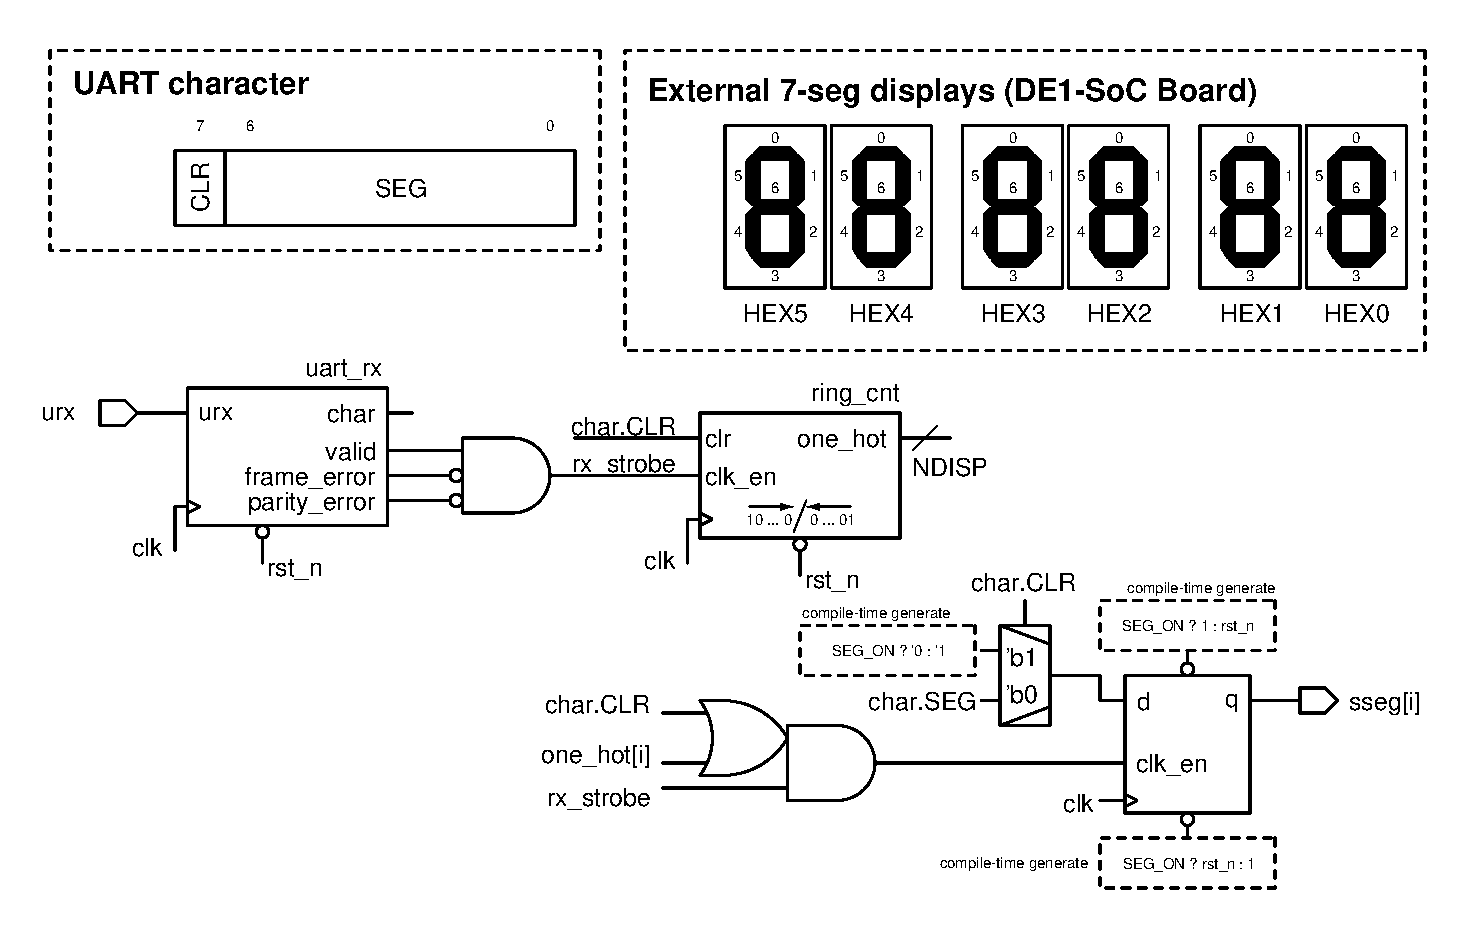
\includegraphics[width=.8\linewidth]{../gfx/display_peripheral.eps}
    \caption{Display peripheral design. The module circularly displays an UART character stream on a set of 7-segment displays.}
    \label{fig:disp_peripheral}
\end{figure}

The display peripheral is devised to serially control a set of 7-segment displays. It processes a stream of UART characters, where each character can either instruct the peripheral to clear all displays or update the input for a single display; one character after the other, the displays can be all updated in a rotating manner.
The design, shown in~\cref{fig:disp_peripheral}, makes use of a custom UART receiver module. When a transmission completes without frame or parity errors, the character appears on the output while the valid signal pulses high: the most significant bit of the character is decoded as the clear command. If the bit is set, the registers driving the display segments are forced into the off-state specified at compile-time, and the one-hot counter is cleared. Otherwise, the one-hot counter state is used to mask all clock-enable signals of the registers driving the display segments, except for one. This register is loaded with the received character data, while the one-hot counter shifts to point to the next display in the set.

\subsubsection{UAR(T) Core}

\begin{listing}
\inputminted{c}{../code/uart_RX.asm}
\caption{Pseudocode of the asynchronous receive operation for the ASM design metodology}
\label{lst:uart}
\end{listing}

The core implements a flexible asynchronous serial receiver for the NRZ-L encoding. It supports several compile-time programmable parameters:
\begin{itemize}
    \item Frame format:
    \begin{itemize}
        \item Character length
        \item Presence and type of parity (even or odd)
        \item Number of STOP bits
    \end{itemize}
    \item Baud rate, by specifying system clock, prescaler, and target clock frequency
    \item Serial line synchronizer depth, which determines the trade-off between data latency and \ac{mtbf} due to metastable events
\end{itemize}
In addition, it features clock synchronization on all transitions, besides the UART-mandated synchronization on the START bit.
Upon reception, the valid signal pulses high for one clock cycle, while the received character and error flags are latched on the outputs.

The module has been designed according to the ASM methodology, starting from the pseudocode in~\cref{lst:uart}; the resulting ASM chart and data path are provided in~\cref{apx:uart}.
 
\subsection{Bipolar Stepper Motor Drive Circuit}\label{subsec:motor_bd}

For educational purposes, the drive circuit does not employ fully integrated bipolar motor drivers. Instead, the L298 integrates two full-bridges to energize and reverse the phase currents. Additionally, the L6506 addresses the limitations of the simpler L/nR drive topology, in which the time constant of the inductive load is reduced by adding external resistances in series with the coils, while the desired asymptotic current is restored by increasing the drive voltage. To avoid the large power dissipation of the external resistances, the approach involves increasing the slew rate of the phase currents with an higher drive voltage, and limiting the phase currents by switching the driver. As shown in~\cref{fig:motor_bd}, the phase current is sensed on the return path from the H-bridge. During the low time of the oscillator period, the drive signals pass through. However, if the phase current exceeds the limit set by the reference voltage, the drive signals are gated for the remaining part of the period. The energy stored in the inductor is dissipated as the current recirculates in the lower half of the bridge: through one snubber diode, the coil resistance, the transistor in the opposite branch, and the sense resistance. Notice that, being possible to independently set the peak phase currents, this chopping circuit supports a microstepping drive technique.

The power output stage of the L298 operates from a fixed \qty{12}{\V} switching power supply~\cite{pwr}. By means of the $(R_5,\,R_6)$ divider, the enable signal pulls low as the supply voltage is about to turn on or off~\cite[9]{l298}. Considering the input characteristics and accounting for a sensible noise margin, it must hold:
\begin{gather*}
    V_\text{IH}+N_\text{MH} \leq V_\text{s}\,\frac{R_6}{R_5+R_6} \leq V_\text{ss} \\
    \frac{V_\text{s}}{R_5+R_6} \gg I_\text{IH}
\end{gather*}
To ensure that the enable signal pulls low in the widest range of the voltage supply dynamic, and assuming a \qty{5}{\percent} tolerance on the resistances, the nominal values in the E12 series can be chosen as:
\begin{align*}
&R_5 = \qty{5.6}{\kohm} &R_6 = \qty{1.8}{\kohm}
\end{align*}

The bipolar stepper motor 17HE15-1504S is rated for a phase current of \qty{1.5}{\A}, and is characterized by a coil resistance of \qty{2.3(.23)}{\ohm} and a coil inductance of \qty{4(.8)}{\mH}. Working with a \qty{10}{\percent} derating factor, the current driven by the L298 is limited to \qty{1.35}{\A} per channel: in the worst case of a total saturation voltage $V_\text{CEsat} = \qty{4.9}{\V}$, the total power dissipated by the driver amounts to \qty{13.23}{\W}.
Now, for the multiwatt15 package in free air, the temperature at the junction would rise above the ambient temperature by:
\[
    \Delta T = R_{\theta\text{ja}}\;P_\text{tot} \approx \qty{463}{\celsius}
\]
hence, the need to lower the thermal resistance with an heat sink. Common heat sinks for this form factor are made of 6063-T5 aluminum alloy, which has a typical thermal conductivity $\kappa$ of \qty{209}{\W\per{\m\kelvin}} (for instance, \cite{xsd_hs}). From the mechanical data of the package, the minimum contact area $S$ to the heat sink is \qty{338.1}{\milli\meter\squared}; therefore, the thermal resistance across the contact area, for an average thickness $\Delta l$ of \qty{5.52}{\milli\m} is:
\[
    R_{\theta\text{sa}} = \frac{\Delta l}{\kappa S} \approx \qty{78.2e-3}{\celsius\per\W}
\]
Finally, by using a thermal compound to improve the thermal coupling between the case and the heat sink, it is reasonable to achieve:
\[
    R_{\theta\text{cs}} \approx \qty{0.5}{\celsius\per\W}
\]
In conclusion, the driver is expected to work at a maximum ambient temperature of:
\[
    T_{\text{a,max}} = T_{\text{j,max}} 
        - \pqty*{R_{\theta\text{jc}}+R_{\theta\text{cs}}+R_{\theta\text{sa}}}
        \;P_\text{tot} \approx \qty{83}{\celsius}
\]
which covers the broadly accepted range for consumer electronics from \qtyrange{0}{70}{\celsius}.

For the current recirculation paths, the datasheet advises selecting fast-switching snubber diodes, preferably of Schottky type. A family of suitable devices is the SB2x0~\cite{sb260}, which are rated for a maximum average forward current of \qty{2}{\A}. As a first approximation, the supply voltage of the power output stage, plus one forward voltage drop of the snubber diode during clamping, bounds the maximum reverse voltage. As a consequence, the SB220 can be selected for the circuit.

The sense resistors must be sized to comply with the maximum allowable voltage at the sensing pins, equal to \qty{2}{\V}. Considering a \qty{680(6.8)}{\mohm} resistor rated for \qty{2}{\W}~\cite{rsense}, the nominal voltage drop for the chosen maximum phase current of \qty{1.35}{\A} is \qty{918}{\mV}. In this condition, the resistor dissipates \qty{1.24}{\W}: computing the thermal resistance from the power derating curve in the datasheet:
\[
    R_\theta = \frac{\qty{155}{\celsius}-\qty{70}{\celsius}}{\qty{2}{\W}}
             = \qty{42.5}{\celsius\per\W}
\]
it is possible to evaluate the effect of self-heating. In the worst case of the \qtyrange{0}{70}{\celsius} temperature range, the resistor heats to:
\[
    T_\text{r,max} = T_{\text{a,max}} + R_\theta\;P \approx \qty{123}{\celsius}
\]
Consequently, from the temperature coefficient $\alpha = \qty{300}{\ppm\per\celsius}$:
\[
    \Delta R_\text{sh} = R_0\,\alpha\,\pqty*{T_\text{r,max} - T_\text{r}0}
    \approx \qty{19.9}{\mohm}
\]
which shows that the self-heating effect dominates the uncertainty. Accordingly:
\[
    R_7 = R_8 = \qty{680(27)}{\mohm}
\]

The sensed voltage is used in the L6506 to implement the constant current drive. In the worst case, the phase current reaches the maximum value of \qty{1.35}{\A} and the sensed voltage at the comparator input is \qty{882}{\mV}. As a consequence, the major constraints are:
\begin{gather*}
    V_\text{ss}\,\frac{R_4}{R_3+R_4} \leq \qty{882}{\mV} \\
    \frac{V_\text{ss}}{R_3+R_4} \gg I_\text{IB}
\end{gather*}
Having already derated the maximum phase current, the constraint can be evaluated for the nominal resistance values. An optimal selection is:
\begin{align*}
    &R_3 = \qty{22}{\kohm} &R_4 = \qty{4.7}{\kohm}
\end{align*}
In fact, with \qty{1}{\percent} uncertainties, the worst case voltage reference would be \qty{895}{\mV}, which corresponds to a maximum phase current of \qty{1.37}{\A}.
In addition, the phase current may exceptionally increase above the chosen peak value during the active time of the oscillator waveform, as the driving inputs cannot be masked. With the same selection of $(R_2,\,C_4)$ as in the application circuit~\cite[5]{l6506}, the nominal frequency of the oscillator is \qty{16.9}{\kHz} and the nominal active time lasts \qty{2.57}{\micro\s}.


\section{Software Design}\label{sec:sw_design}

Prototyping with STM32 microcontrollers is facilitated by the STM32Cube project, which aims to simplify development by providing a comprehensive embedded software platform for each STM32 series. This software kit is complemented by the STM32CubeMX tool~\cite{cubemx}, which enables the graphical configuration of the peripherals and the clock tree of the microcontroller, as well as the automatic generation of the corresponding initialization code in the C language.

Given the opportunity to gain a deeper understanding of the tools involved in the cross-platform build process, but also to achieve greater control and flexibility over the firmware architecture, the software project is structured from scratch using CMake, without relying on STM32CubeMX. The details of the buildsystem are discussed in~\cref{subsec:buildsys}.

To benefit from the object-oriented and generic programming paradigms, the firmware is developed in \cpp. The software architecture follows a bare metal yet layered design, with a clear separation between virtualized hardware resources and application logic. Depending on the resource, the virtualization is implemented in one of two ways:
\begin{itemize}
    \item As an object, with public methods directly invoked by the application. 
    \item As a file, manipulated through I/O library functions or system calls.  
\end{itemize}
This latter approach is typical of UNIX-like systems, where special files are interfaces to device drivers, and the \ac{vfs} makes the association between the low-level operations invoked internally by file-related system calls and their implementation in the drivers. Accordingly, the firmware includes a custom implementation of a minimal virtual file system, which is presented in~\cref{subsec:files}. The device drivers and the simpler objects abstracting hardware resources are covered in~\cref{subsec:vdev}.

The firmware also relies on the following generic abstraction layers:
\begin{itemize}
    \item The \acsu{cmsis} Core(M) component, which provides a standardized API for all Arm Cortex-M processor cores. It consists of two complementary parts:
    \begin{itemize}
        \item The Core(M) Standard, delivered as a set of vendor-independent C header files directly by Arm. It declares the core exception vectors and defines the functions for accessing core and core peripheral registers, special CPU instructions, and the SIMD instructions.

        \item The Core(M) device, developed by the silicon vendor, in this case, STMicroelectronics. It declares interrupt vectors and defines the functions for startup and system configuration.

        Note that the startup assembly code provided by STMicroelectronics is not used in this project; it is replaced by a \cpp version tailored to a custom linker script.
    \end{itemize}

    \item The STM32Cube \ac{ll} drivers~\cite{UM1725}, which offer a lightweight and portable C abstraction to operate directly on memory-mapped peripheral registers. Whenever convenient, this abstraction is extended in the project with utility functions at the same abstraction level, organized by peripheral in dedicated namespaces (e.g., \icpp{dma::}, \icpp{exti::}, \icpp{flash::}).

    \item The newlib nano and GNU standard \cpp libraries. Newlib nano is a size-optimized variant of newlib, an ANSI C standard library implementation intended for use on embedded systems; it is prebuilt and distributed with the Arm GNU Toolchain.
\end{itemize}

\subsection{The Buildsystem}\label{subsec:buildsys}

CMake acts as a meta-build tool that translates an abstract buildsystem written in the CMake language into configuration files for the native build tool of the host platform.
To support cross-compilation, CMake is told about the target platform via a toolchain file. For this project, this is found split into:
\begin{description}
    \item[\itxt{arm-none-eabi.cmake}] It provides basic configuration settings for an AArch32 bare metal target. It establishes the cross-compilation environment by automatically locating the Arm GNU Toolchain installation in the host platform and defines compiler and linker options optimized for embedded development.
    In addition, it introduces interface targets corresponding to different C/\cpp runtime variants: 
    \begin{itemize}
        \item \itxt{ARM::FreeStanding} for standalone applications which do not use the standard startup files and libraries.
        \item \itxt{ARM::NoSys} for bare metal applications to weakly link system calls with stubs that implement graceful failure.
        \item \itxt{ARM::Newlib} for linking with newlib C and GNU \cpp standard libraries.
        \item \itxt{ARM::Nano}, \itxt{ARM::Nano::FloatPrint}, \itxt{ARM::Nano::FloatScan} to refine the size-optimizations of the newlib C standard library being linked.
    \end{itemize}

    \item[\itxt{armv7em-hard-fpv4sp.cmake}] It specializes the generic configuration of AArch32 bare metal targets for the Armv7-M architecture profile, also enabling the \ac{dsp} and single-precision \ac{fp} extensions. The settings are encapsulated in the interface target \itxt{ARM::V7EM-HARD-FPV4SP}.
\end{description}

\begin{listing}
\begin{minted}{text}
MEMORY
{
  FLASH (rx)  : ORIGIN = 0x08000000, LENGTH = 16K*4 + 64K + 128K*2
  NVS   (w!x) : ORIGIN = 0x08060000, LENGTH = 128K
  RAM   (w!x) : ORIGIN = 0x20000000, LENGTH = 96K
}
\end{minted}
\caption{Location and size of the memory blocks available in the \mcu target, described in the linker command language.}
\label{lst:ld_script}
\end{listing}
    
At the top level, the \itxt{CMakeLists.txt} configures project-specific settings. It loads the toolchain file, specifies the linker script, and collects the project sources and the external libraries to link with.
The linker script is a key component of the build process, as it describes how the sections in the input object files are mapped into the output executable file, and what its memory layout is.
The \mcu microcontroller is equipped with \qty{96}{\kibi\byte} of static RAM and \qty{512}{\kibi\byte} of NOR flash memory, which is partitioned in eight erasable sectors as follows: four \qty{16}{\kibi\byte} sectors, one \qty{64}{\kibi\byte} sector, and three \qty{128}{\kibi\byte} sectors. To allow for the non-volatile retention of the movement pattern, the load script reserves a dedicated memory region matching the last \qty{128}{\kibi\byte} flash sector, as shown in~\cref{lst:ld_script}.

The linker script is also tightly connected to the startup file. On system reset, the vector table is expected at address \texttt{0x00000000}, with the stack pointer reset value in its first entry. The linker ensures that this placement is satisfied and provides the stack pointer reset value, and several other addresses referenced by the code, by means of symbol definitions. Specifically, the linker script manages all the space left in the SRAM region as a shared ascending-heap/descending-stack: the start address of the region initializes the variable used to track the top of the heap in the \icpp{_sbrk()} system call, which handles heap allocation; whereas the end address of the region is put in the first vector table entry.
Other symbols are referenced while setting up the runtime context: the \icpp{Reset_Handler()} initializes the \itxt{data} segment in the SRAM by copying from the flash, according to the addresses provided by the linker; similarly, the C/\cpp initialization code makes use of these addresses to clear the \itxt{bss} segment, and to locate the initialization and de-initialization routines.

\subsection{Virtual File System}\label{subsec:files}

In general, hiding complexity behind simple and uniform interfaces is highly desirable. In UNIX-like systems, resources are abstracted as files, allowing user applications to interact with them using the same system calls as for regular files (e.g., \icpp{open()}, \icpp{read()}, \icpp{write()}, etc.). This framework relies on the \ac{vfs}, which defines a common set of low-level operations supported by all file types. These operations are invoked internally by system calls, and dispatched to their implementation depending on the file type. In particular, for special files representing character devices, the implementation of the file operations is provided by the corresponding device driver, a C kernel module that exposes the hardware as a byte stream, hiding its actual behavior.

Given the number of peripherals behaving as character devices in the project, the firmware implements a lightweight abstraction layer to support file-related system calls. This is achieved through the \icpp{IFile} and \icpp{FileManager} classes.
\begin{description}
    \item[\icpp{class IFile}] It is the abstract base class that defines the interface to operate on files. A device driver is thus a derived class that overrides the supported operations; by default, all operations are implemented in \icpp{IFile} to return the error code \icpp{-ENOSYS}.
    
    \item[\icpp{class FileManager}] It implements relevant file system services using the data structures illustrated in~\cref{fig:fm_datastr}.
    Special files are represented as \icpp{Node} objects, namely links between a file name and a driver object. The full list of special files is specified at compile time via the file manager constructor, which forwards it to initialize the node table member, as shown in~\cref{fig:node_table}.
    The open file table tracks open files at run time. As depicted in~\cref{fig:ofile_table}, each entry of this data structure holds a pointer to a node along with state data; file descriptors index the open file table and are considered free when the corresponding entries hold no valid node pointer.
    
    \begin{figure}
      \centering
      \subfloat[][Compile-time table of nodes: each entry links the name of the file representing a character device to its corresponding driver.\label{fig:node_table}]{
        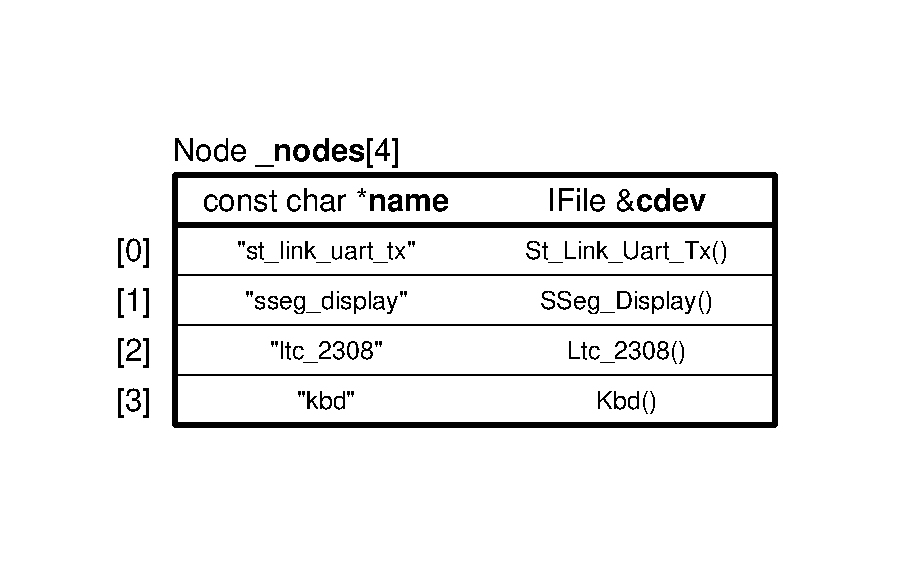
\includegraphics[width=0.45\linewidth]{../gfx/NodeTable.eps}
      }
      \qquad
      \subfloat[][Run-time table of open files, indexed by file descriptors: an open file entry holds a pointer to the associated node and some state data.\label{fig:ofile_table}]{
        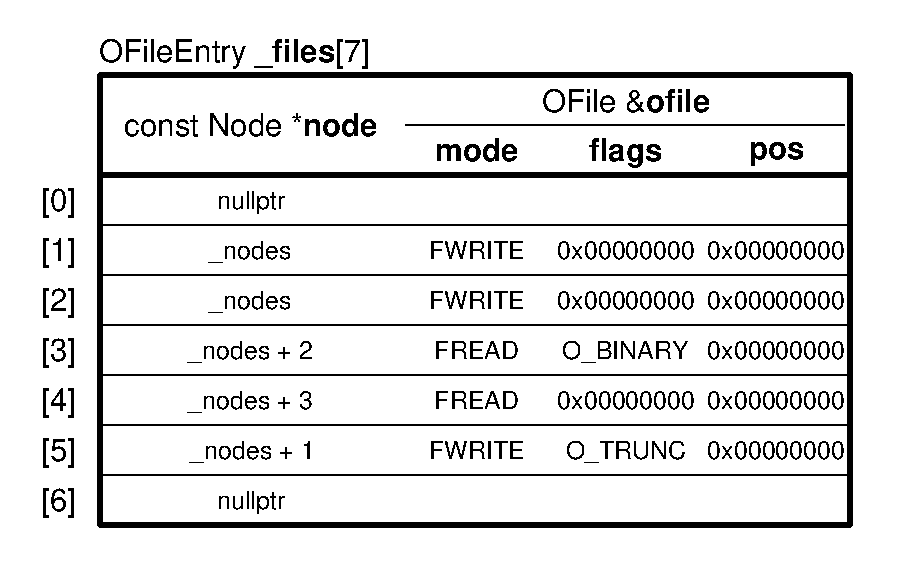
\includegraphics[width=0.45\linewidth]{../gfx/OFileTable.eps}
      }
      \caption{\icpp{FileManager} data members}
      \label{fig:fm_datastr}
    \end{figure}
    
    The file system services roughly follow POSIX semantics:
    \begin{itemize}
        \item \icpp{open()} performs name resolution through the node table to locate the associated node object. It then allocates the lowest, non-reserved file descriptor shown free in the open file table and initializes the corresponding open file table entry with the address of the node, as well as the access mode and the flags passed as arguments. Finally, the driver implementation of the operation is invoked via the node object.

        \item \icpp{close()} reverses the actions of \icpp{open()}, provided that the file descriptor identifies an open file. The driver implementation of the operation is invoked via the node pointer, which is retrieved in the open file table entry indexed by the file descriptor. Afterward, the file descriptor is released by invalidating the node pointer.

        \item \icpp{lseek()}, \icpp{read()}, and \icpp{write()} follow a similar pattern: if the file descriptor refers to an open file, the corresponding driver operation is invoked via the node pointer from the open file table.
        The only exception is that \icpp{read()} and \icpp{write()} check that the access mode specified when opening the file is compatible with the requested operation.

        \item \icpp{select()} enables monitoring multiple file descriptors for readiness to perform an I/O operation without blocking.
        Internally, for each monitored file descriptor referring to an open file, the ready state is questioned with the driver \icpp{poll()} operation, invoked via the node pointer from the open file table.
    \end{itemize}
\end{description}

\subsection{Virtualized Resources}\label{subsec:vdev}

The firmware follows two approaches when dealing with hardware resources:
\begin{itemize}
    \item Behavior close to microcontroller peripherals capabilities is abstracted through \cpp classes that directly expose a convenient interface of public member functions to the application code. This is discussed in~\cref{ssubsec:obj}.
    
    \item Behavior of complex hardware devices that fit a byte-stream access model is abstracted through device drivers, relying on the virtual file system layer.
    Note that, in all cases, device parameters are not manipulated through \icpp{ioctl()} calls, but directly with the methods exposed by the drivers.
    The device drivers are presented in~\cref{ssubsec:cdev}.
\end{itemize}

\subsubsection{Object Abstractions}\label{ssubsec:obj}

\paragraph{\mintinline[fontsize=\normalsize]{cpp}{class HwAlarm}}
It transforms a free-running general-purpose timer into an interrupt-based alarm scheduler and a delay generator.

The class is parameterized with the timer base address, allowing to refine its implementation at compile-time, based on the features of the chosen timer: namely, the width of the counter, and the number of independent capture/compare channels.
The channels are abstracted as an array of \icpp{Alarm} objects, which hold the parameters representing a runnable alarm on the corresponding channel. The representation consists of: a pointer to a callback functor, which differentiates between running alarms when valid and free channels; the remaining number of repetitions, and the periodicity converted to counter ticks.
Note that the implementation relies on the \icpp{ICallback} abstract base class to provide an interface to non-owning functor wrappers of function and member function pointers.

The setup is performed by the \icpp{init()} method. It computes the prescaler to achieve the desired counter clock resolution, then it enables the interrupt request in the \ac{nvic}, and the timer in free-running mode.

When the \icpp{setAlarm()} method is invoked to set up a new alarm, the caller specifies how many times it will fire, the periodicity, and the callback functor. Provided that there are free channels and that the periodicity is representable in the counter width, a free \icpp{Alarm} entry is initialized with the alarm parameters. The target compare value is computed starting from the current counter tick and is used to configure the corresponding capture/compare channel for interrupt generation on match events. When the interrupt fires and the handler starts executing, the triggered alarms are identified, their representation is updated, and lastly their callback functors are invoked for execution.

The \icpp{delay()} method provides traditional blocking delays, capable of exceeding the counter reload period. This is implemented through a polling loop that accumulates the elapsed time since function invocation, and compares it against the target delay.

\paragraph{\mintinline[fontsize=\normalsize]{cpp}{class PushButton}}
It implements an interrupt-based push button handler, with debouncing logic and short/long press detection.

\begin{figure}
    \centering
    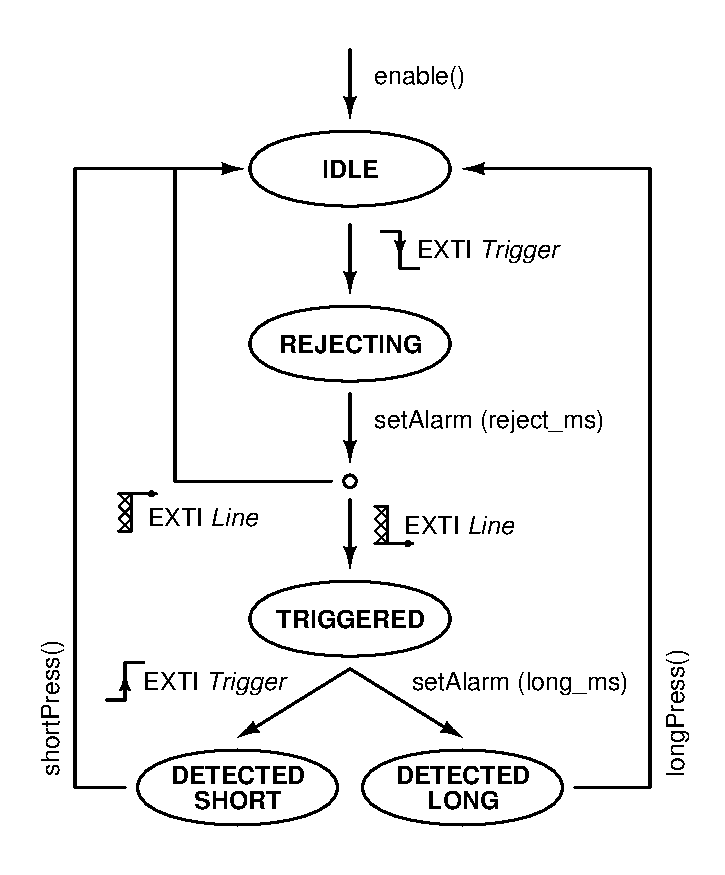
\includegraphics[width=.45\linewidth]{../gfx/PushButton_fsm.eps}
    \caption{\icpp{PushButton} internal FSM for an active low push button}
    \label{fig:pb_fsm}
\end{figure}

The class behavior follows the FSM illustrated in~\cref{fig:pb_fsm}, where the key state transitions are driven either by external edge-sensitive interrupts or by alarm timeouts. 
The application is supposed to query the button state with the \icpp{shortPress()} and \icpp{longPress()} methods, which are non-blocking and return \icpp{true} when the corresponding gesture is detected.

\paragraph{\mintinline[fontsize=\normalsize]{cpp}{class BStepper}}
It generates the waveforms required to drive the windings terminals of a bipolar stepper motor, supporting both full-step and half-step modes. This is achieved with minimal CPU overhead by delegating the transfer of precomputed bit patterns onto the GPIO port via a DMA controller, synchronized by the advanced hardware timer.

\begin{figure}
    \centering
    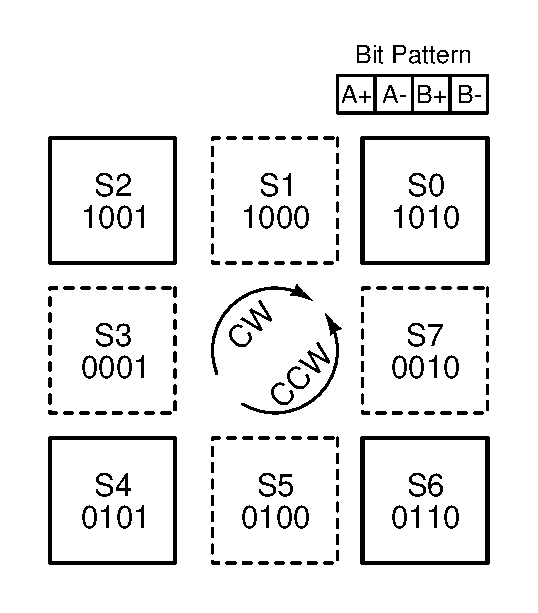
\includegraphics[width=.35\linewidth]{../gfx/Translator_states.eps}
    \caption{Bipolar motor phase states for \acs{cw} and \acs{ccw} rotations; the dashed states are skipped in full-step mode.}
    \label{fig:bsteps}
\end{figure}

Provided that the windings terminals belong to the same GPIO port, a bit pattern can be fully represented as a \ac{bsrr} mask on \qty{32}{\bit}. Given the motor phase states shown in~\cref{fig:bsteps}, the \icpp{Translator} class generates four arrays of bit patterns corresponding to \ac{cw} and \ac{ccw} driving sequences in half-step and full-step modes.
While the half-step and full-step sequences consist of eight and four states respectively, the corresponding bit pattern arrays are twice as long. This redundant data simplifies the DMA transfer, which occurs from a memory region handled as a circular buffer targeting the GPIO \ac{bsrr}. This is because the \icpp{Translator} class tracks the motor phase state as an index within the half-step sequence, ranging from \numrange{0}{7}. Without this redundancy, locating the start address of the circular buffer by simply indexing the masks arrays with a state number for half-step movements, and half that value for full-step movements, could result in out-of-bounds accesses.

The initializations of GPIO pins, DMA controller, advanced timer, and \ac{nvic} are performed by the \icpp{init()} method. The advanced timer is configured in up-counting mode, with overflows as the only source of \acp{uev}.

Motor movements are initiated with the \icpp{rotate()} method and require no further intervention from the CPU, except when the number of steps minus one does not fit in the \ac{rcr} of the advanced timer.
As a preliminary step, the \icpp{calcTimeBase()} method determines the values for the prescaler and auto-reload registers, such that the reload period matches the step duration, and the counter resolution is numerically lowest. That is
\[
    \pqty*{\text{PSC}+1}\,\pqty*{\text{ARR}+1} = \nint*{{f_\text{PSC}}\;T_\text{s}}
\]
where the step duration $T_\text{s}$ is expressed as
\[
    T_\text{s} = \frac{\qty{60}{\s\per\minute}}{N\;\omega_\text{rpm}}
\]
with $N$ being the motor resolution in steps per revolution, and $\omega_{\text{rpm}}$ the rotational frequency in revolutions per minute.

\begin{figure}
    \centering
    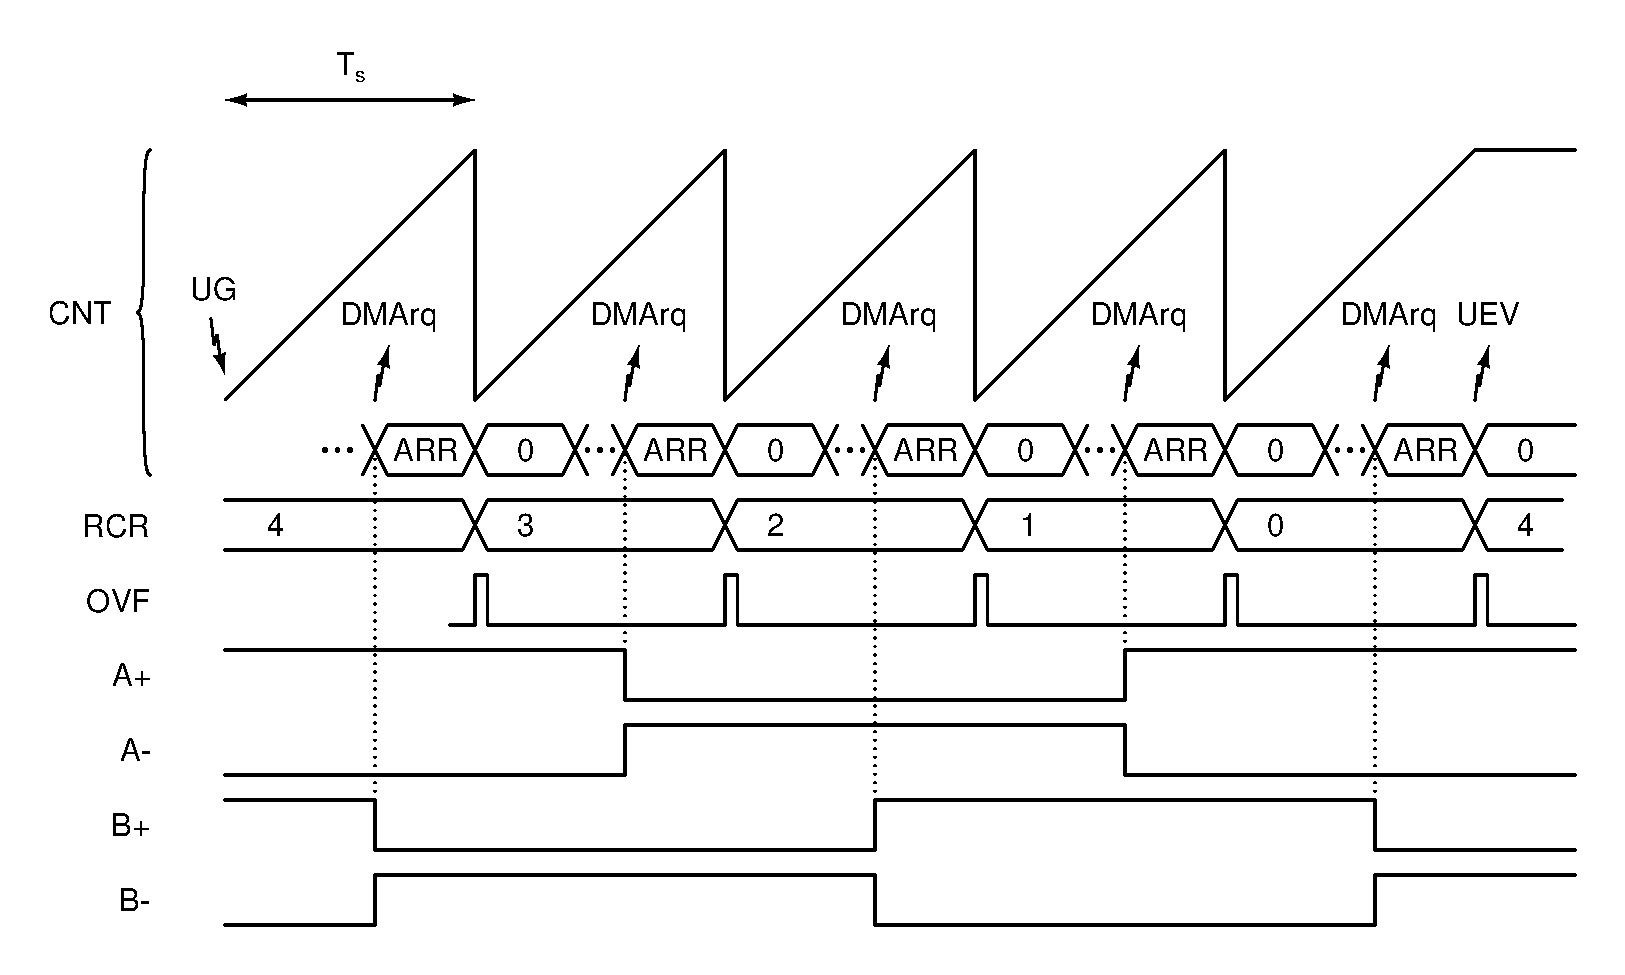
\includegraphics[width=\linewidth]{../gfx/BStepper_run.eps}
    \caption{\icpp{BStepper::rotate()} execution diagram for the simpler case when the number of steps fits the \acs{rcr}. Starting from the motor phase state S0, the motor takes five full steps in \acs{ccw} direction.}
    \label{fig:bstep_run}
\end{figure}

Considering the simpler case when the number of steps minus one fits the \ac{rcr}, the core logic is the following.
The \ac{rcr} is forcefully loaded with a software \ac{uev} and the counter is configured in one pulse mode.
The \icpp{Translator::advance()} method updates the internal motor phase state to reflect the one at the end of the movement. In addition, it locates the start address of the circular buffer with the precomputed sequence of \ac{bsrr} masks, which is used to reconfigure the DMA stream source. The last configuration step determines when to generate the DMA requests: one capture/compare channel of the advanced timer is configured to fire the requests on match events, with a compare value equal to the auto-reload register. Finally, the counter is enabled: as an example of the resulting execution diagram, see~\cref{fig:bstep_run}. 

If this approach is not feasible, the \ac{rcr} is set to its maximum value and the hardware-counted repetitions are supplemented with software-counted ones (namely, \ac{rcr} reload events). Except for the corner case where exactly one software repetition must be counted, this is handled by starting the advance timer with the one pulse mode disabled. It is configured such that, upon counter overflow and \ac{rcr} reload, the \ac{uev} generates an interrupt. The handler then updates the software repetitions count and, in the last software-counted cycle, either preloads the \ac{rcr} or directly switches the counter to one pulse mode. In the former case, at the end of the software repetitions count, the counter is switched to one pulse mode as well.

\paragraph{\mintinline[fontsize=\normalsize]{cpp}{class MotionPattern}}

It implements an \icpp{std::vector}-like container for \icpp{MotionSegment} objects, that is allocated in a flash sector with wear-levelling and cached in SRAM over a statically allocated array.

The class is parameterized by the maximum number of elements it can contain.
While the elements stored in the SRAM array are plain \icpp{MotionSegment} objects, the corresponding flash entries are instances of a larger type, \icpp{FlashChunkEntry}, which packs an additional byte attribute that indicates whether the entry is valid (\icpp{WRITTEN = 0xAA}) or not (\icpp{ERASED = 0xFF}).

As it happens in the application, suppose that the class allocates the non-volatile container in the \qty{128}{\kibi\byte} sector starting at address \texttt{0x08060000} and that the \icpp{FlashChunkEntry} is represented on \qty{8}{\byte}. If the maximum number of elements is taken to be four, then the sector can accomodate
\[
    N = \frac{\qty{128}{\kibi\byte}}{\text{\icpp{sizeof(FlashChunkEntry[4])}}} = 4096
\]
distinct containers, hence the logical partitioning of the sector into corresponding $N$ chunks. The wear-levelling mechanism leverages this excess space to minimize the number of sector erasures. Clearing the non-volatile container does not immediately cause a sector erase; instead, it invalidates the current chunk and enables the next one available. This process continues until all chunks have been invalidated, only then the sector is erased. To illustrate, consider~\cref{fig:mp}:
\begin{enumerate}[label=\textbf{(\alph*)}]
    \item Starting in the erased state, the container is located in the first chunk and has a zero size; entry zero is pointed to be the written next.
    \item After three write operations, the container is still located in the first chunk. The fourth entry is pointed to be written next.
    \item The container is cleared: the chunk is invalidated by marking the first entry as \icpp{DIRTY = 0x00}. The container is now located in the second chunk and entry zero is pointed to be written next.
    \item After $N-1$ clear operations, all chunks are marked dirty but the last one. A further clear operations triggers a sector erase.
\end{enumerate}

\begin{figure}
    \centering
    \subfloat[][Fully erased sector, empty container\label{fig:mp_ff}]{
        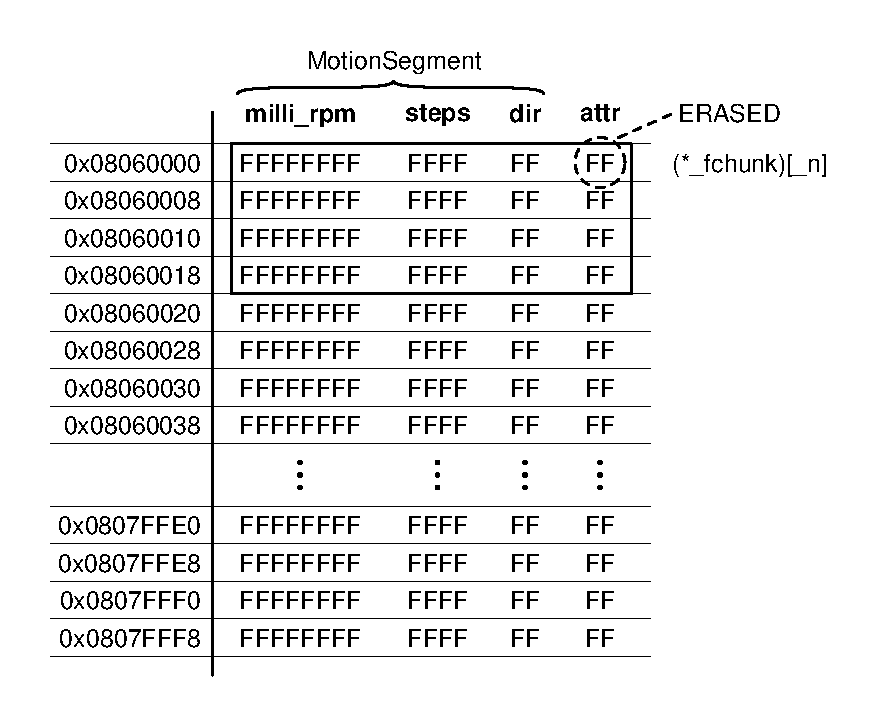
\includegraphics[width=.47\linewidth]{../gfx/MotionPattern_ERASED.eps}
    }\hfill
    \subfloat[][First chunk in use, container size is three\label{fig:mp_wr}]{
        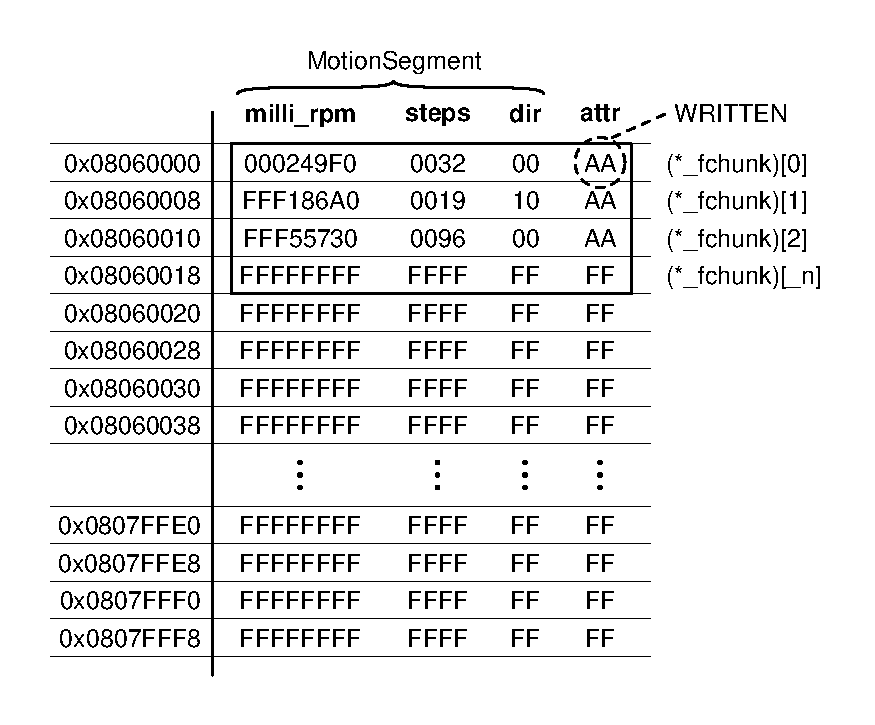
\includegraphics[width=.47\linewidth]{../gfx/MotionPattern_WRITTEN.eps}
    }\\
    \subfloat[][First chunk marked dirty, second chunk in use, container is empty\label{fig:mp_dy}]{
        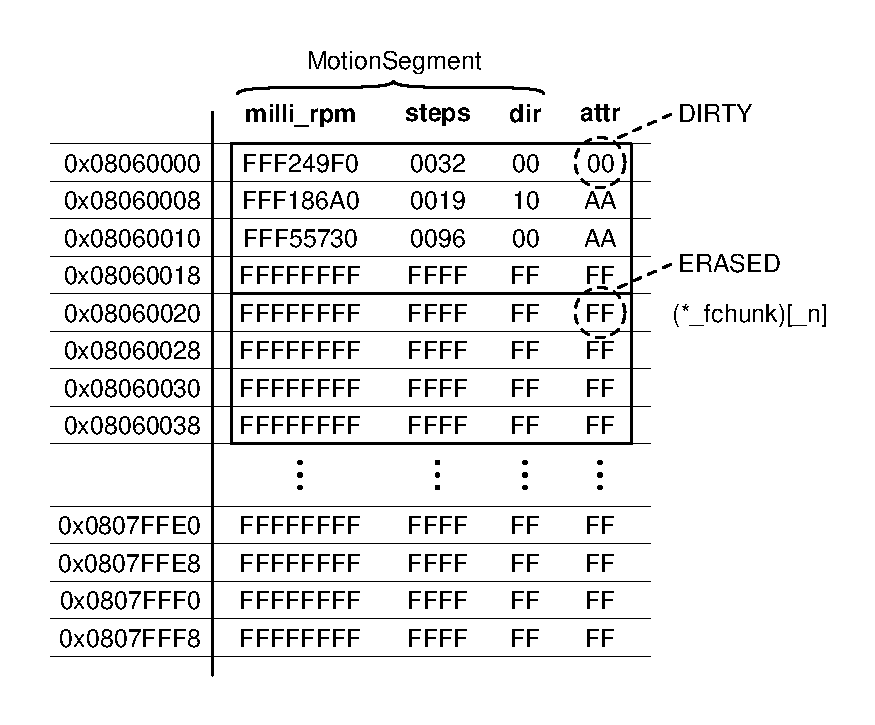
\includegraphics[width=.47\linewidth]{../gfx/MotionPattern_DIRTY.eps}
    }\hfill
    \subfloat[][All chunks marked dirty but the last one in use. Clearing the container triggers a sector erase.\label{fig:mp_te}]{
        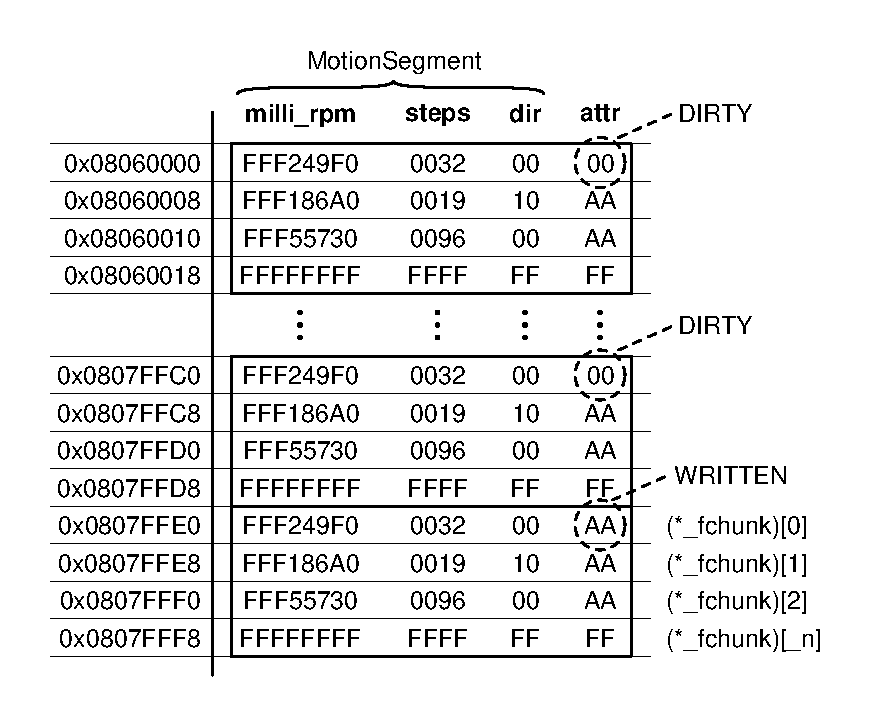
\includegraphics[width=.47\linewidth]{../gfx/MotionPattern_TOERASE.eps}
    }
    \caption{\icpp{MotionPatter} logic for managing the persistence of the \icpp{MotionSegment[4]} array.}
    \label{fig:mp}
\end{figure}

\paragraph{\mintinline[fontsize=\normalsize]{cpp}{class SpiMaster}}

It provides a simple interface to communicate with multiple SPI slave devices, internally managing the select-signal generation via GPIO.

During initialization, the GPIO pins assigned to \acsu{sclk}, \acsu{mosi}, and \acsu{miso} are configured in the alternate function corresponding to SPI. Since these pins are left floating when the controller is disabled, weak pull-downs are enabled. The SPI controller is configured as well, preparing for master-mode, full-duplex operation with software-managed slave selection.

The communication targets are abstracted as an array of \icpp{Slave} objects, each holding the protocol parameters and the GPIO pin to be used for slave selection. Targets are dynamically registered via the class interface: provided that there are free entries in the array of targets, the \icpp{addSlave()} method computes the lowest prescaler that satisfies the requested \ac{sclk} maximum frequency, and stores the SSN pin information and protocol parameters. It returns the index of the newly registered slave, which serves as its identifier. 
Although the \mcu SPI peripheral supports only \qty{8}{\bit} and \qty{16}{\bit} transfers, the class accommodates arbitrary frame lengths up to \qty{16}{\bit} by adjusting the alignment of the transmitted and received data.

Full-duplex transfers are blocking and are performed with the \icpp{txrx()} method specifying the identifier of the target slave. If the retrieved slave-dependent configuration differs from the last active one, the SPI controller is reconfigured accordingly. Note that, in this case, the configuration of weak pull-up/down resistors on \ac{sclk} is changed to match the clock polarity required by the slave. 
Then the method asserts the SSN line, generates a pre-transfer delay via the \icpp{HwAlarm} abstraction, executes the transfer, and de-asserts the SSN line after a post-transfer delay. 

\subsubsection{Device Drivers}\label{ssubsec:cdev}

\paragraph{\mintinline[fontsize=\normalsize]{cpp}{class UartTx}}

It is a lightweight driver for the USART peripheral, implementing DMA-based UART transmission in blocking or non-blocking fashion.

The driver object is configured directly through its public methods, which includes assigning a GPIO pin, a DMA stream, and protocol parameters like frame settings and baud rate. Note that the character payload has a fixed length of \qty{8}{\bit}.

The initialization of the underlying peripherals is performed when opening the device file, which supports only the write mode. The DMA stream is prepared for a memory-to-peripheral direct byte transfer: the source address points to the start of the characters buffer and is auto-incremented by the DMA controller; the destination is fixed and corresponds to the data register of the USART peripheral. On the USART side, following the configuration of the protocol parameters, the DMA transmission mode is enabled.

The implementation of the \icpp{write()} operation is trivial. If there is an ongoing transfer, the open-file flags are queried to determine if it is acceptable to block while waiting for it to complete. Upon completion, the user data buffer is copied locally, the DMA stream is enabled, and the transmission continues with no further intervention from the CPU.

\paragraph{\mintinline[fontsize=\normalsize]{cpp}{class SSegDisplay}}

It is the driver for the display peripheral presented in~\cref{subsec:sseg}, implemented by extending the generic capabilities of the \icpp{UartTx} base class with functionalities such as character re-encoding, text buffering, and interrupt-based text scrolling.

In addition to the configuration of the base driver object, the method \icpp{setDisplay()} allows to configure the number of 7-segment displays composing the peripheral screen, the minimum number of times a string that does not fit on the screen should be scrolled, and the scrolling speed.
The alphabet supported by the peripheral is built at compile time via the template function \icpp{fmtChar()} and made available for the re-encoding of an ASCII stream through the private method \icpp{encode()}.

Opening the device file performs the same initialization described for the base class, with the only peculiarity that truncation forces the driver to transmit a \icpp{CLEAR} command to the peripheral.

\begin{figure}
    \centering
    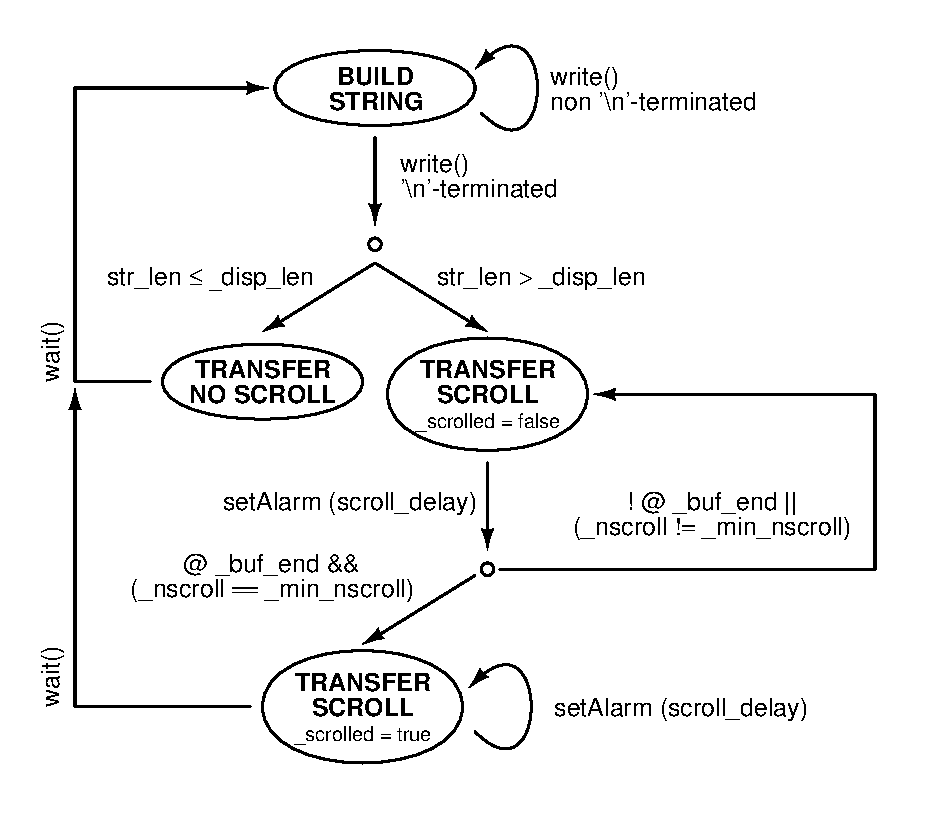
\includegraphics[width=.6\linewidth]{../gfx/SSegDisplay_fsm.eps}
    \caption{\icpp{SSegDisplay} internal FSM for text scrolling}
    \label{fig:sseg_fsm}
\end{figure}

At the core of the \icpp{write()} method there is the agreement that the newline character indicates the termination of a string to be transmitted. It is expected that the text may exceed the screen length, hence the implementation of an interrupt-based mechanism to handle the scrolling of the displayed text. This is achieved in collaboration with the \icpp{HwAlarm} class, following the FSM illustrated in~\cref{fig:sseg_fsm}, where the state transitions are driven either by application logic or by alarm timeouts.

It is worth noting that when the driver is scrolling a string, the alarm callback is executed by the \icpp{HwAlarm} object within an interrupt handler. Since the UART transfer is synchronized via DMA, the amount of processing required in CPU Handler Mode is minimal. This holds true except when the last contiguous substring has been transmitted to the peripheral, in which case a \icpp{std::rotate()} operation is performed to manipulate the underlying character buffer and produce the effect of continuous scrolling.

\paragraph{\mintinline[fontsize=\normalsize]{cpp}{class LTC2308}}

It is a full driver for the ADC peripheral discussed in~\cref{subsec:adc}, implemented according to the timing diagrams and the applications information found in the datasheet~\cite{ltc2308}.

The class collaborates with the \icpp{SpiMaster}, in charge of the low-level details of SPI communication, and with the \icpp{HwAlarm}, that generates the delays required to satisfy timing constraints.
The configuration of the driver object includes specifying the protocol-related parameters required for registering a slave with the \icpp{SpiMaster}: these are the \ac{convst} pin, which triggers both the start of the analog-to-digital conversion process and the start of the SPI transfer, and the maximum \icpp{sclk} frequency.
In addition, the \icpp{setOptions()} method internally generates the programming word that configures the actual ADC peripheral, based on the input range type (unipolar or bipolar), the input stage type (single-ended or differential), the multiplexer channels, and the power management mode.

Opening the device file has the effect of registering the slave target with the \icpp{SpiMaster} and transmitting the programming word to initialize the ADC peripheral with the selected options. 
The \icpp{read()} method implements the logic for acquiring a stream of \qty{12}{\bit} samples from the ADC peripheral and transforming it into a binary stream of \qty{16}{\bit} signed or unsigned integers, according to the selected options.

\paragraph{\mintinline[fontsize=\normalsize]{cpp}{class Keyboard}}

It is a full driver for PS/2-compatible keyboards using scan code set 2, interfaced through the custom PS/2-to-SPI peripheral described in~\cref{ssubsec:ps22spi}.

Communication with the SPI slave and timing synchronization are implemented similarly to the \icpp{LTC2308} driver, relying on the \icpp{SpiMaster} and \icpp{HwAlarm} abstractions. The \icpp{SpiMaster::txrx()} function is further abstracted with private helper methods, tailored to the behavior of the peripheral device:
\begin{description}
    \item[\icpp{_pollTxRx()}] Sends a command to the peripheral and polls for an acknowledgment within a bounded number of SPI cycles. This approach is necessary because: first, command execution requires time; second, the full-duplex nature of the transfer implies that data received from the slave cannot represent the response to the command being sent concurrently.

    \item[\icpp{_trySet()}] Builds upon \icpp{_pollTxRx()} to implement the transmission logic of the PS/2 \textit{Set/Reset Status Indicator} command to the keyboard, which consists of a command byte followed by an argument byte. First, an SPI command programs the PS/2 controller in transmit mode to send \texttt{0xED}; the controller is then reconfigured to receive the keyboard's acknowledgment. The process is repeated to transmit the argument byte.
\end{description}

Opening the device file registers the slave with the \icpp{SpiMaster} and issues a reset sequence: inside the peripheral, the PS/2 controller is disabled and re-enabled, and the FIFO buffer is flushed. Then, \icpp{_trySet()} is invoked to turn off both the Num Lock and Caps Lock indicators.

The \icpp{poll()} operation must determine whether a subsequent \icpp{read()} call would return a character, ideally without blocking. In practice, one blocking SPI transfer is performed via the helper method \icpp{_tryRead()} to check if a scan code is available for processing. Note, however, that the presence of a scan code does not guarantee that a character is ready to be returned. This is where the parsing machine comes into play. It consists of:
\begin{description}
    \item[\icpp{class ScanCodeParser}] Implements the logic for parsing the scan codes belonging to set 2 with a FSM and a lookup table. Processing any scan code generates a \icpp{ParsedKey} object, which is differently interpreted based on its \icpp{Action} field. Some scan codes merely advance the FSM without yielding actionable information; these are represented with action \icpp{NONE}. Conversely, the \icpp{MAKE} and \icpp{BREAK} actions are paired with the layout-independent representation of the key for which the make or break code has been received; this is represented as an enumerator of \icpp{UniKey} type.

    \item[\icpp{_map()}] Translates layout-independent \icpp{UniKey} keys into ASCII characters using a layout-specific lookup table, considering the current state of modifier keys (Left/Right Shift, Alt Gr, Caps Lock, and Num Lock).
    
    Note that while the current implementation provides the Italian lookup table, the mapping can be generalized through template parameters and specialization.
    
    \item [\icpp{_step()}] Overall, it implements the logic that translates scan codes into ASCII characters, returning \icpp{'\0'} when the scan code does not yield such information.

    In details, the scan code is first parsed into a \icpp{ParsedKey} object. If the action is \icpp{MAKE} or \icpp{BREAK}, the associated key is processed as follows:
    \begin{itemize}
        \item If it corresponds to a modifier key, the internal state is updated accordingly. For Caps Lock and Num Lock, a small FSM determines whether the corresponding keyboard indicators should be updated, in which case \icpp{_trySet()} is invoked.
        
        \item Otherwise, only key press (corresponding to the \icpp{MAKE} action) requires processing. In this case, the \icpp{_map()} helper function is invoked.
    \end{itemize}
\end{description}
Tying things together: if \icpp{_tryRead()} yields a scan code, it is processed by \icpp{_step()}, which may produce a non-zero character, which updates the internal \icpp{_peek} member. The \icpp{poll()} operation returns accordingly: a \icpp{_peek} value different from \icpp{'\0'} indicates read readiness.

The \icpp{read()} function complements this behavior. If \icpp{poll()} was previously called, the \icpp{_peek} value may already contain a character. If not, and the open file flags allow blocking, a character is fetched using the helper method \icpp{_getc()}, which repeatedly calls \icpp{_tryRead()} and \icpp{_step()} until a valid character becomes available.

\subsection{Main Application}

The application integrates all the described abstractions to implement the theory of operation presented in~\cref{sec:theory_operation}.

Device drivers and objects requiring exception handling follow the \ac{cofu} idiom, which ensures proper initialization order before the \icpp{main()} is run.
System initialization proceeds through several phases, notably:
\begin{itemize}
    \item \icpp{systemClockConfig()} establishes a \qty{64}{\mega\hertz} system clock using the internal RC oscillator and the PLL. The number of wait states for flash memory access is adjusted accordingly.

    \item The logging system is setup using the low-level driver \icpp{UartTx} over USART2, which is accessible through the on-board ST-LINK debugger/programmer. The standard input and standard error streams are redirected to the corresponding device file.

    \item The \icpp{HwAlarm} object is constructed over the general-purpose \qty{16}{\bit} timer TIM9, which features two independent capture/compare channels. The time base is configured with a counter clock frequency of \qty{64}{\kHz}.

    \item The ADC device file is opened for buffered binary reading. The buffer size is configured to \qty{16}{\bit}, so that each \icpp{read()} operation from the driver returns a complete sample.

    \item The display device file is opened for line-buffered writing: due to truncation, the screen is cleared. As the newline character both flushes the buffer and triggers a transmission to the display, the number of \icpp{write()} invocations is minimized.
\end{itemize}

If all initializations are successful, the system performs a sign of life sequence by printing \textit{run...} on the peripheral display and rotating the motor shaft one full turn counterclockwise and back clockwise at \qty{25}{\rpm}.

The main loop is designed following a polling scheme:
\begin{enumerate}
    \item Detection of \icpp{Push_Button().longPress()} is immediately handled to clear the movement pattern.
    
    \item Detection of \icpp{Push_Button().shortPress()} with a non-empty movement pattern is immediately handled to initiate movement pattern execution.
    Similarly, the detection of \icpp{Push_Button().shortPress()} while executing the movement pattern immediately aborts movement pattern execution.
    
    \item Detection of available input from the keyboard through the \icpp{select()} system call is immediately handled to attempt acquisition of a new motion segment.

    Note that keyboard input validation is not implemented using the \cpp standard regex library, which parses and compiles the regular expression pattern at runtime. Resorting to the \textit{Compile Time Regular Expressions} library significantly reduced the program image size while also improving execution speed.
\end{enumerate}


\clearpage
\appendix

\section{PS/2 Controller}\label{apx:ps2_controller}

\rotatebox{90}{
    \begin{minipage}{.85\textheight}
        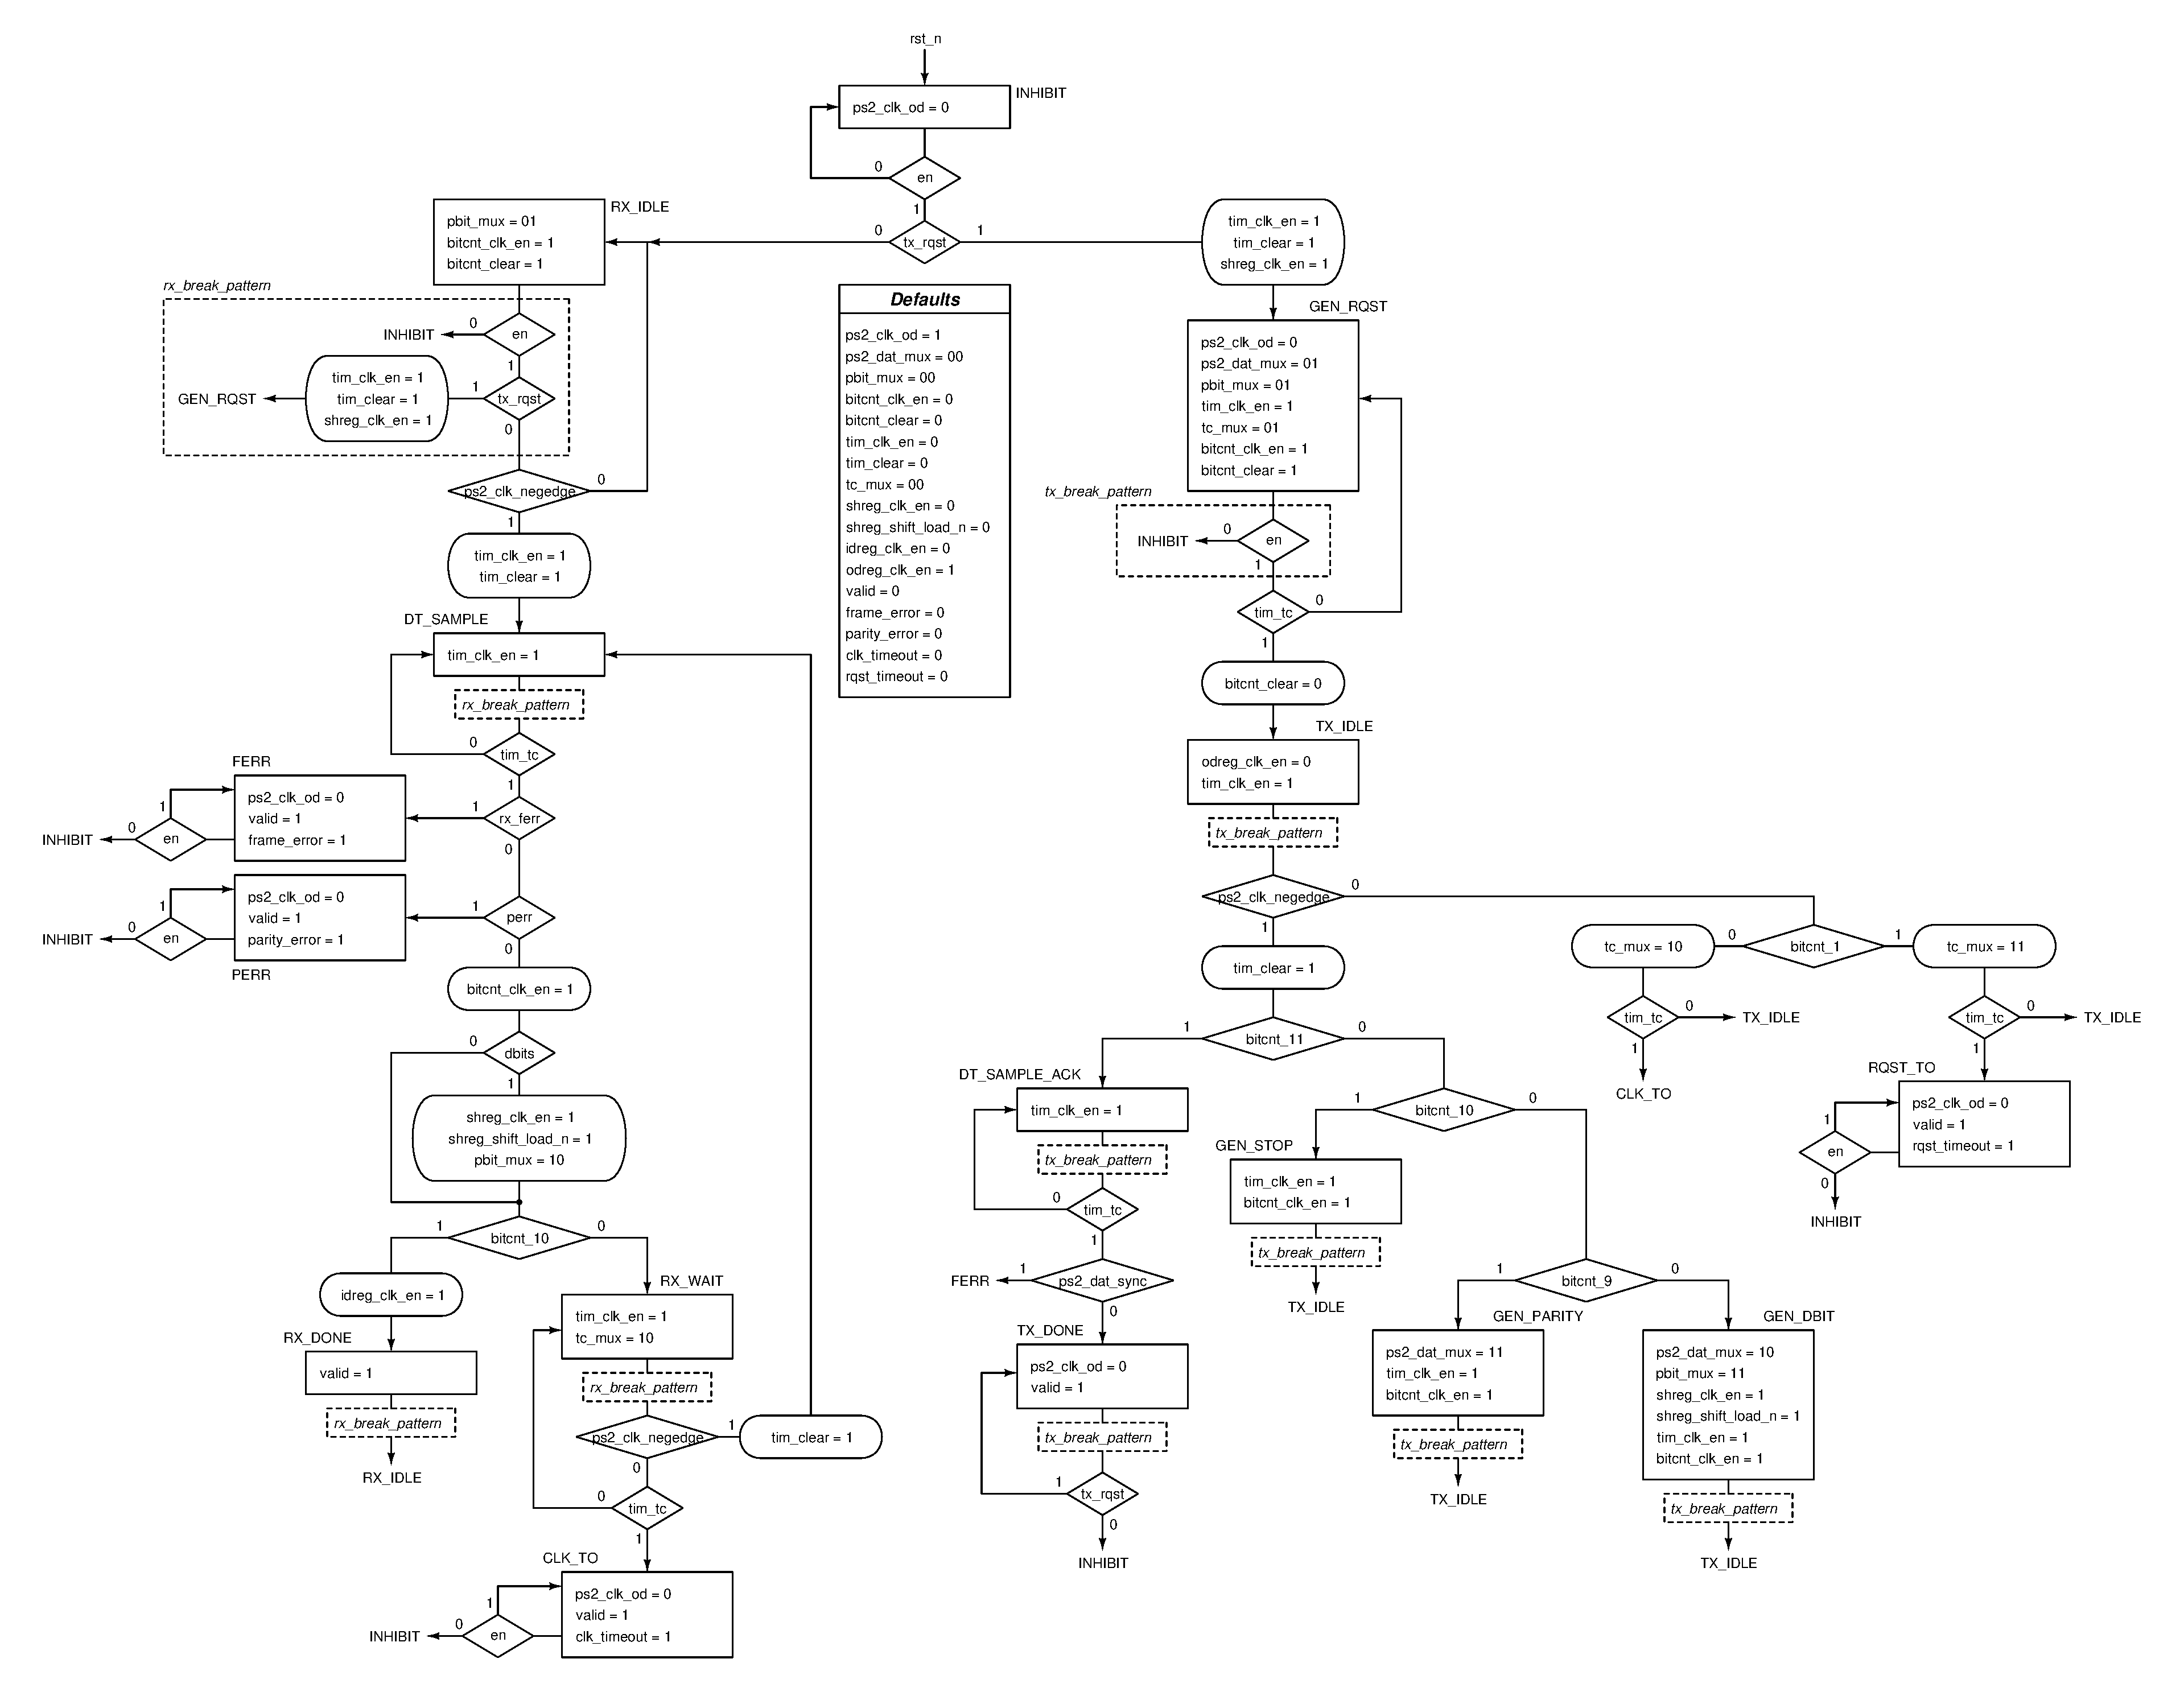
\includegraphics[width=\textwidth]{../gfx/ps2_asm.eps}
        \captionof{figure}{PS/2 controller detailed ASM chart}
        \label{fig:ps2_asm}
    \end{minipage}
}

\rotatebox{90}{
    \begin{minipage}{.85\textheight}
        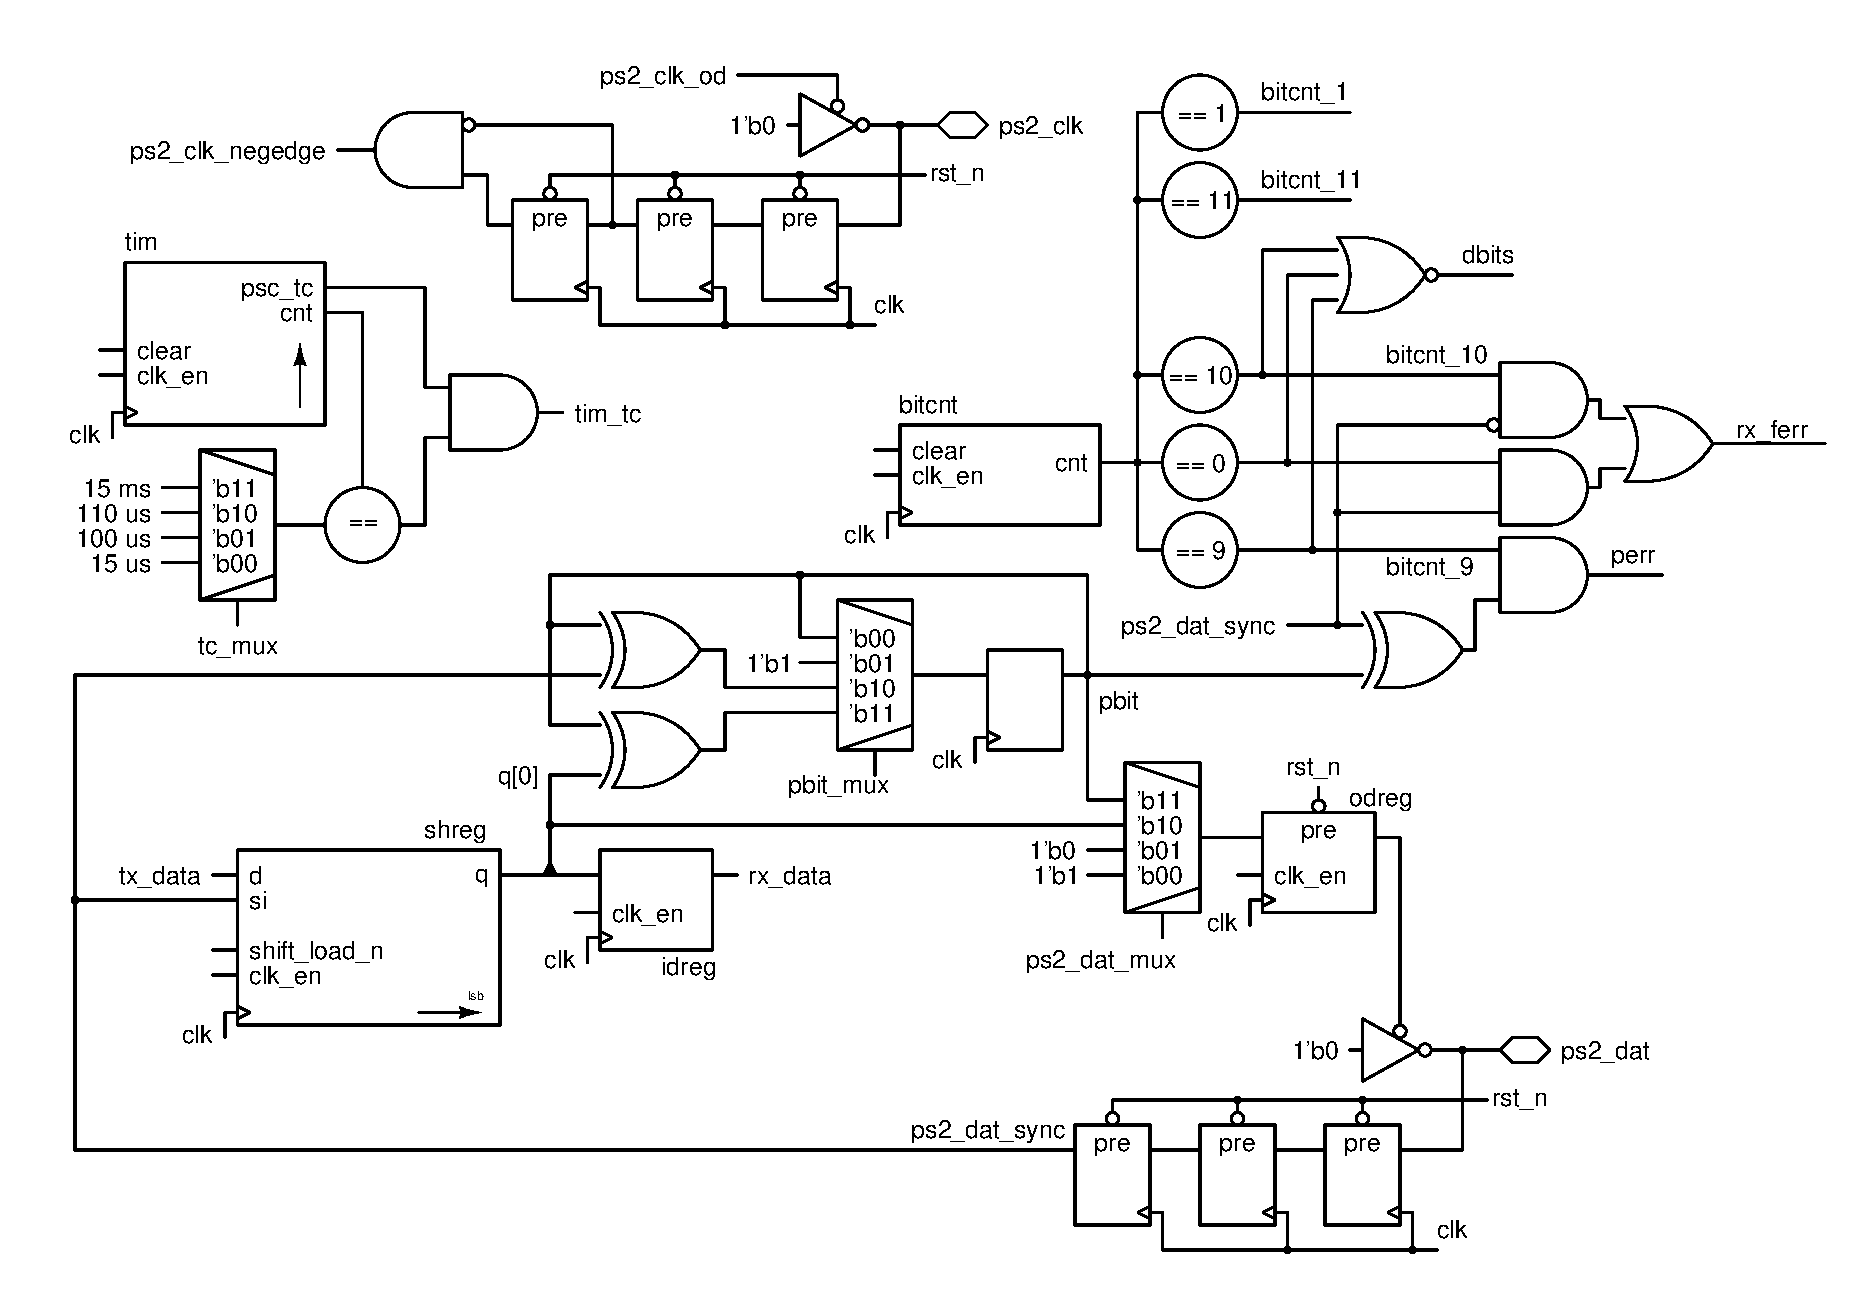
\includegraphics[width=\linewidth]{../gfx/ps2_dp.eps}
        \captionof{figure}{PS/2 controller data path}
        \label{fig:ps2_dp} 
    \end{minipage}
}

\clearpage
\section{Show-Ahead Single-Clock FIFO}\label{apx:fifo}

\begin{center}
    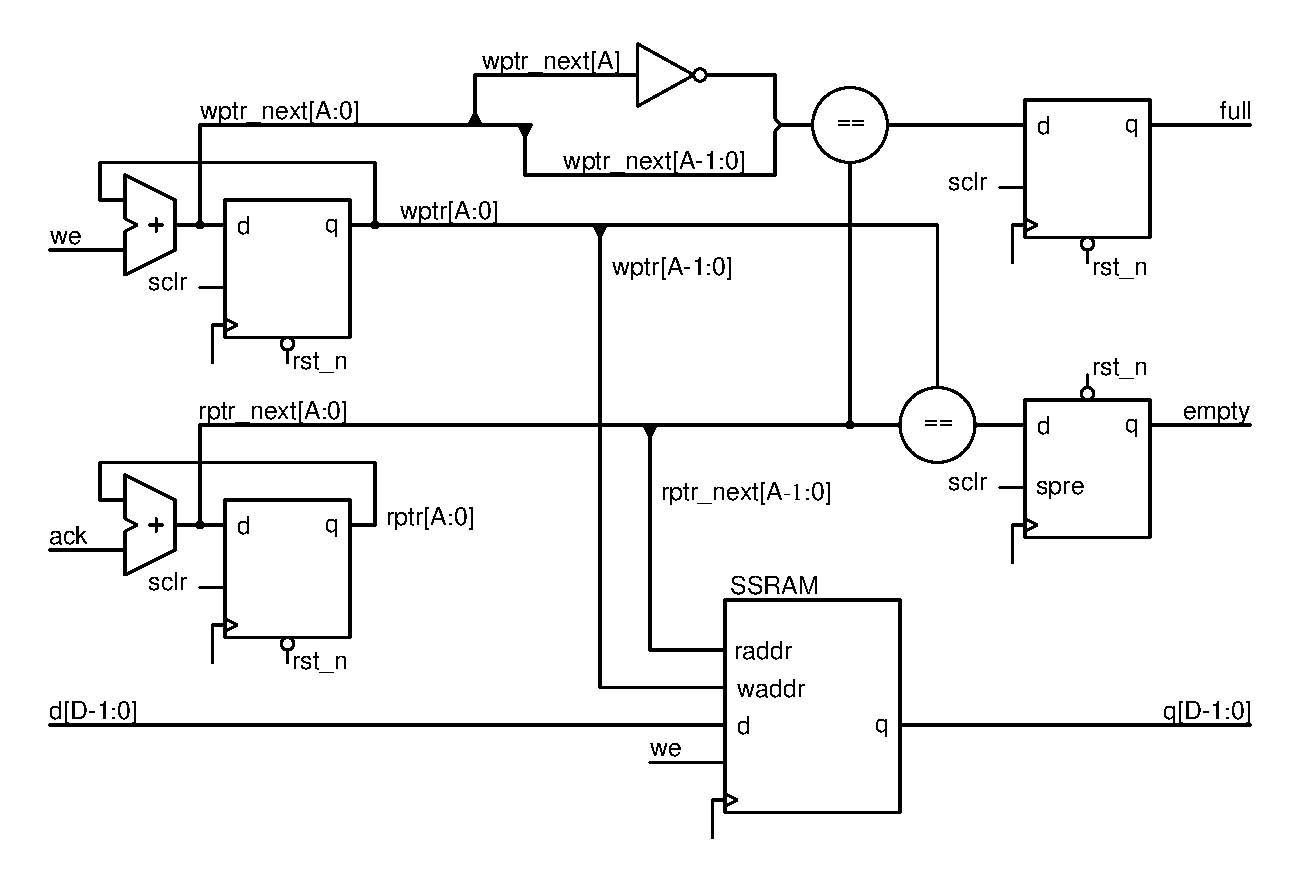
\includegraphics[width=.7\linewidth]{../gfx/fifo.eps}
    \captionof{figure}{Show-ahead single-clock FIFO design}
    \label{fig:fifo}
\end{center}

\section{SPI Slave Controller}\label{apx:spi}

\begin{figure}[h!]
    \centering
    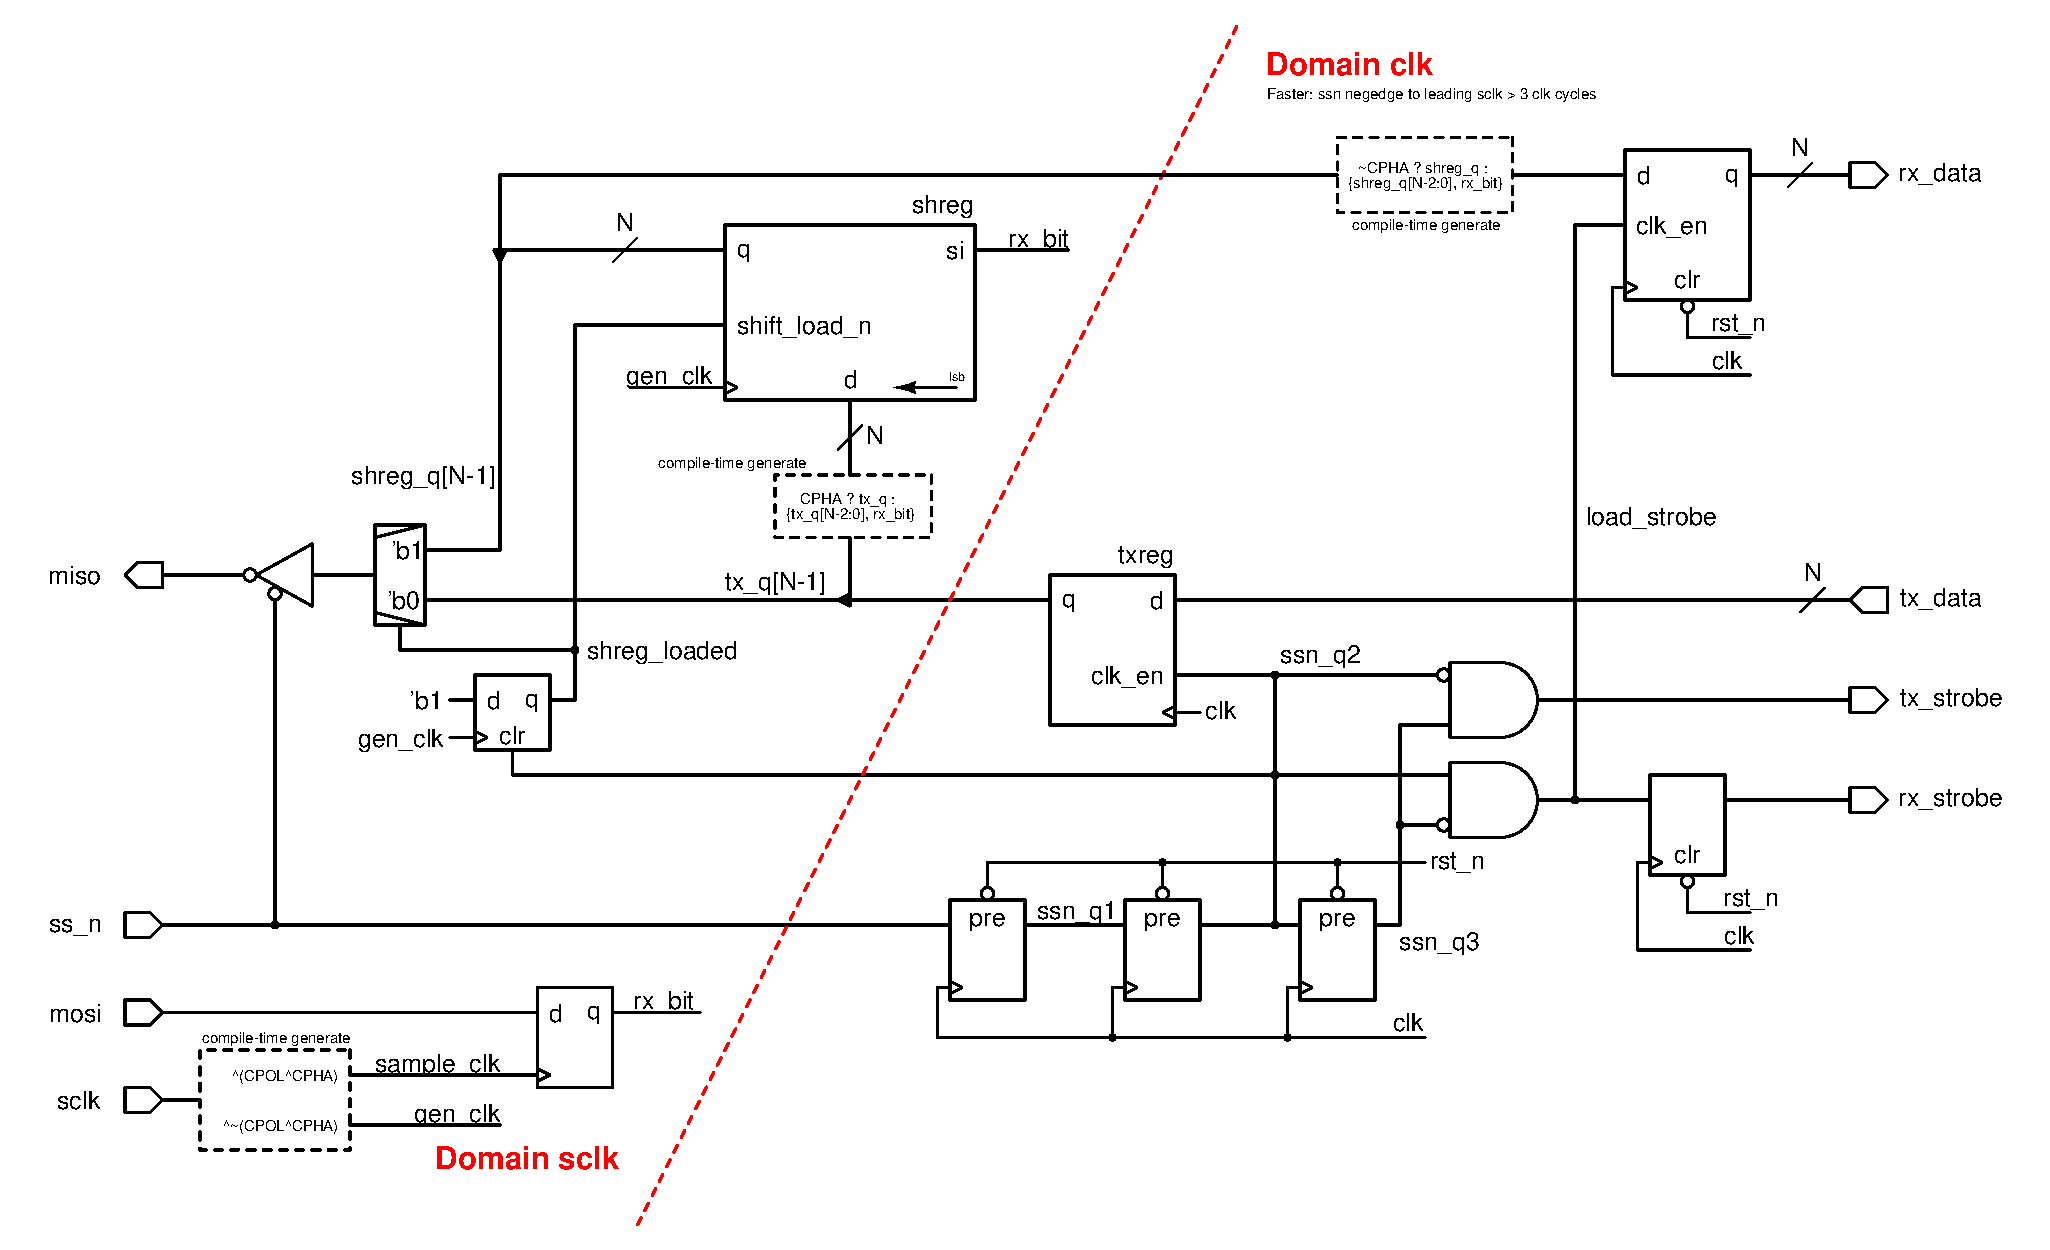
\includegraphics[width=\linewidth]{../gfx/spi_slave.eps}
    \caption{SPI slave controller}
    \label{fig:spi_slave}
\end{figure}

\begin{figure}[h!]
    \centering
    \subfloat[][\qty{4}{\bit} transmission, CPOL = 0, CPHA = 0]{
        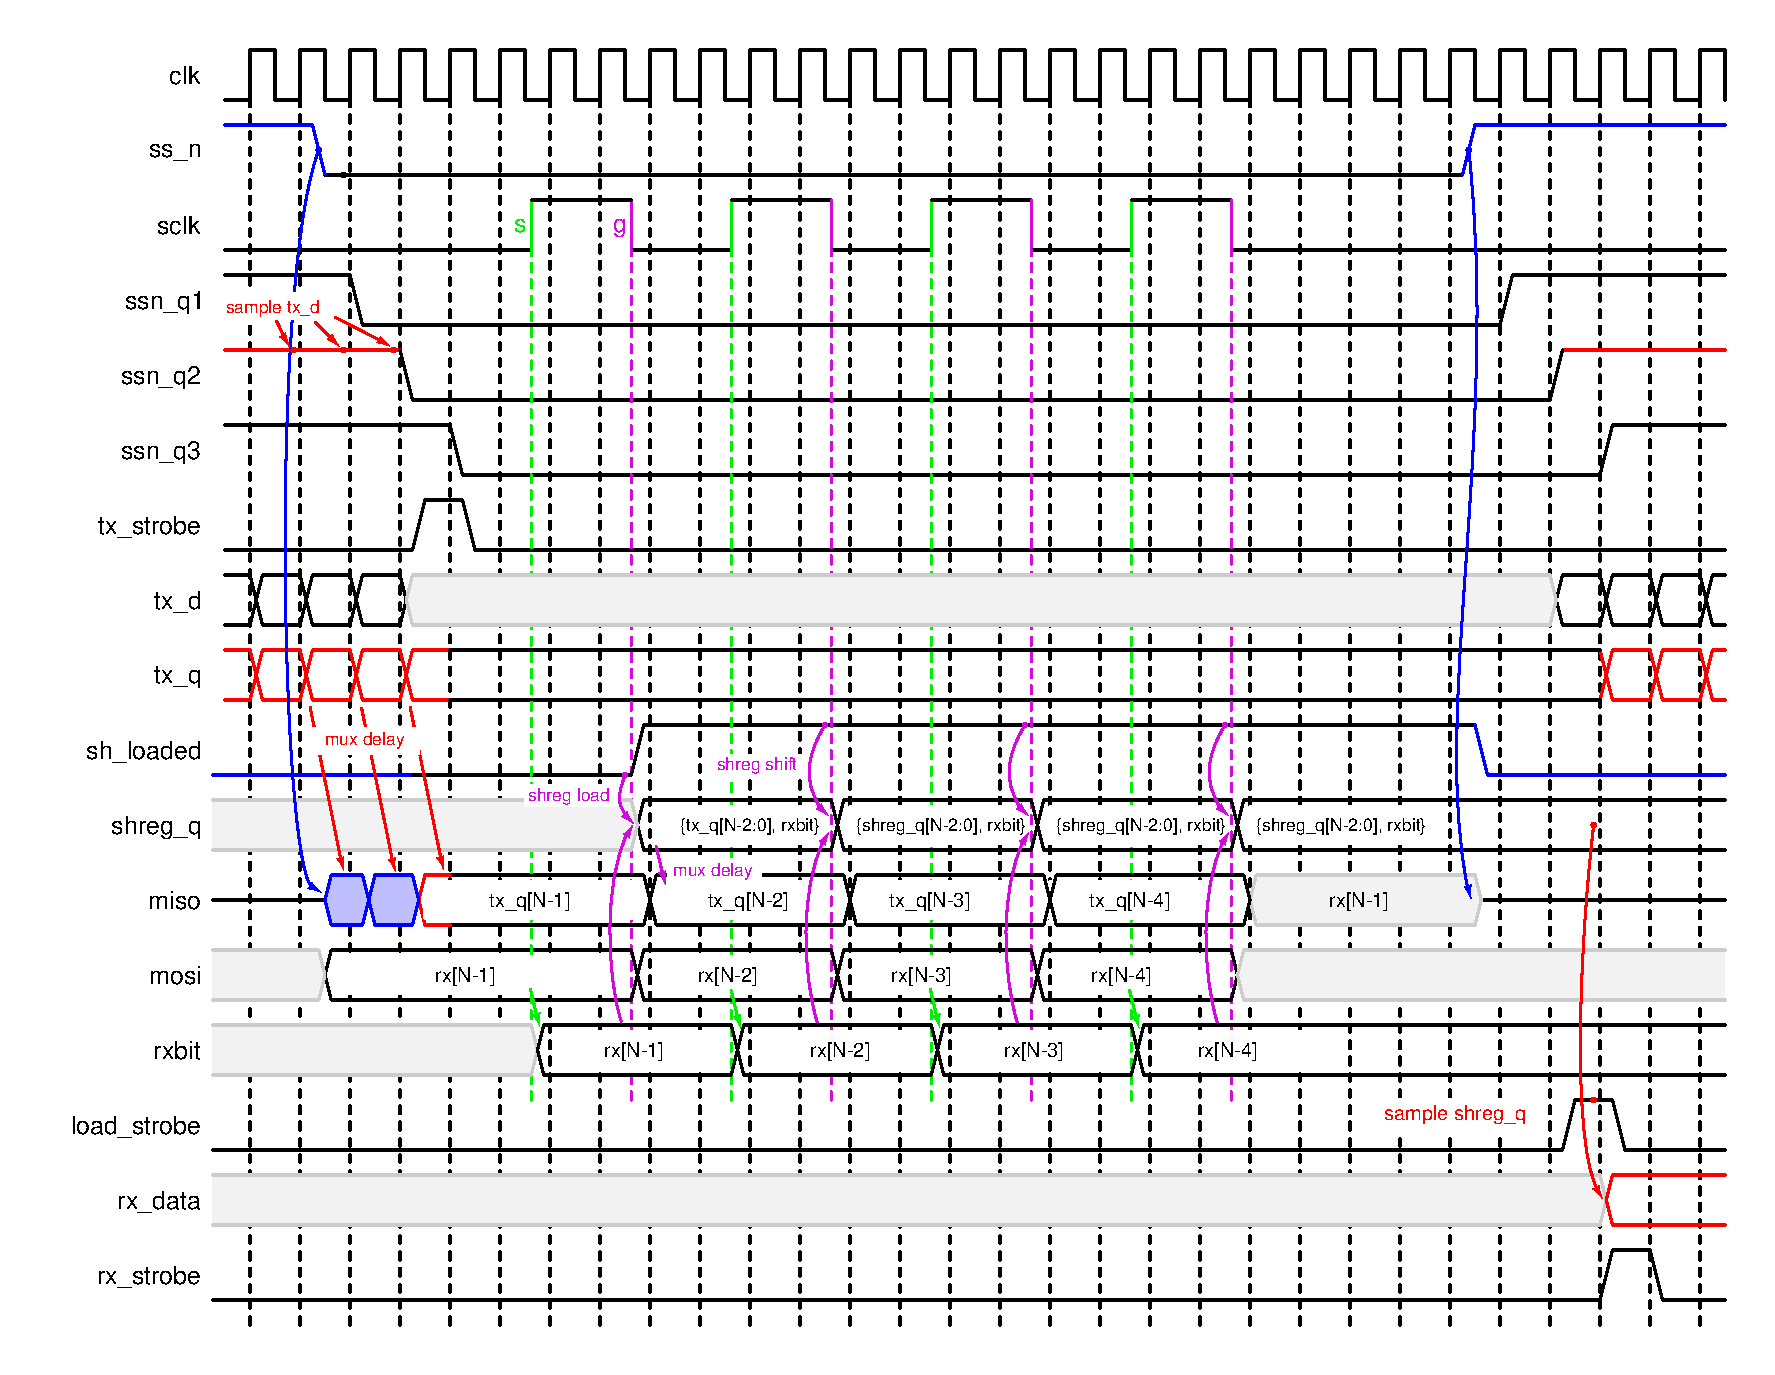
\includegraphics[width=.8\linewidth]{../gfx/spi_timing_cpha0.eps}
    }\\
    \subfloat[][\qty{4}{\bit} transmission, CPOL = 0, CPHA = 1]{
        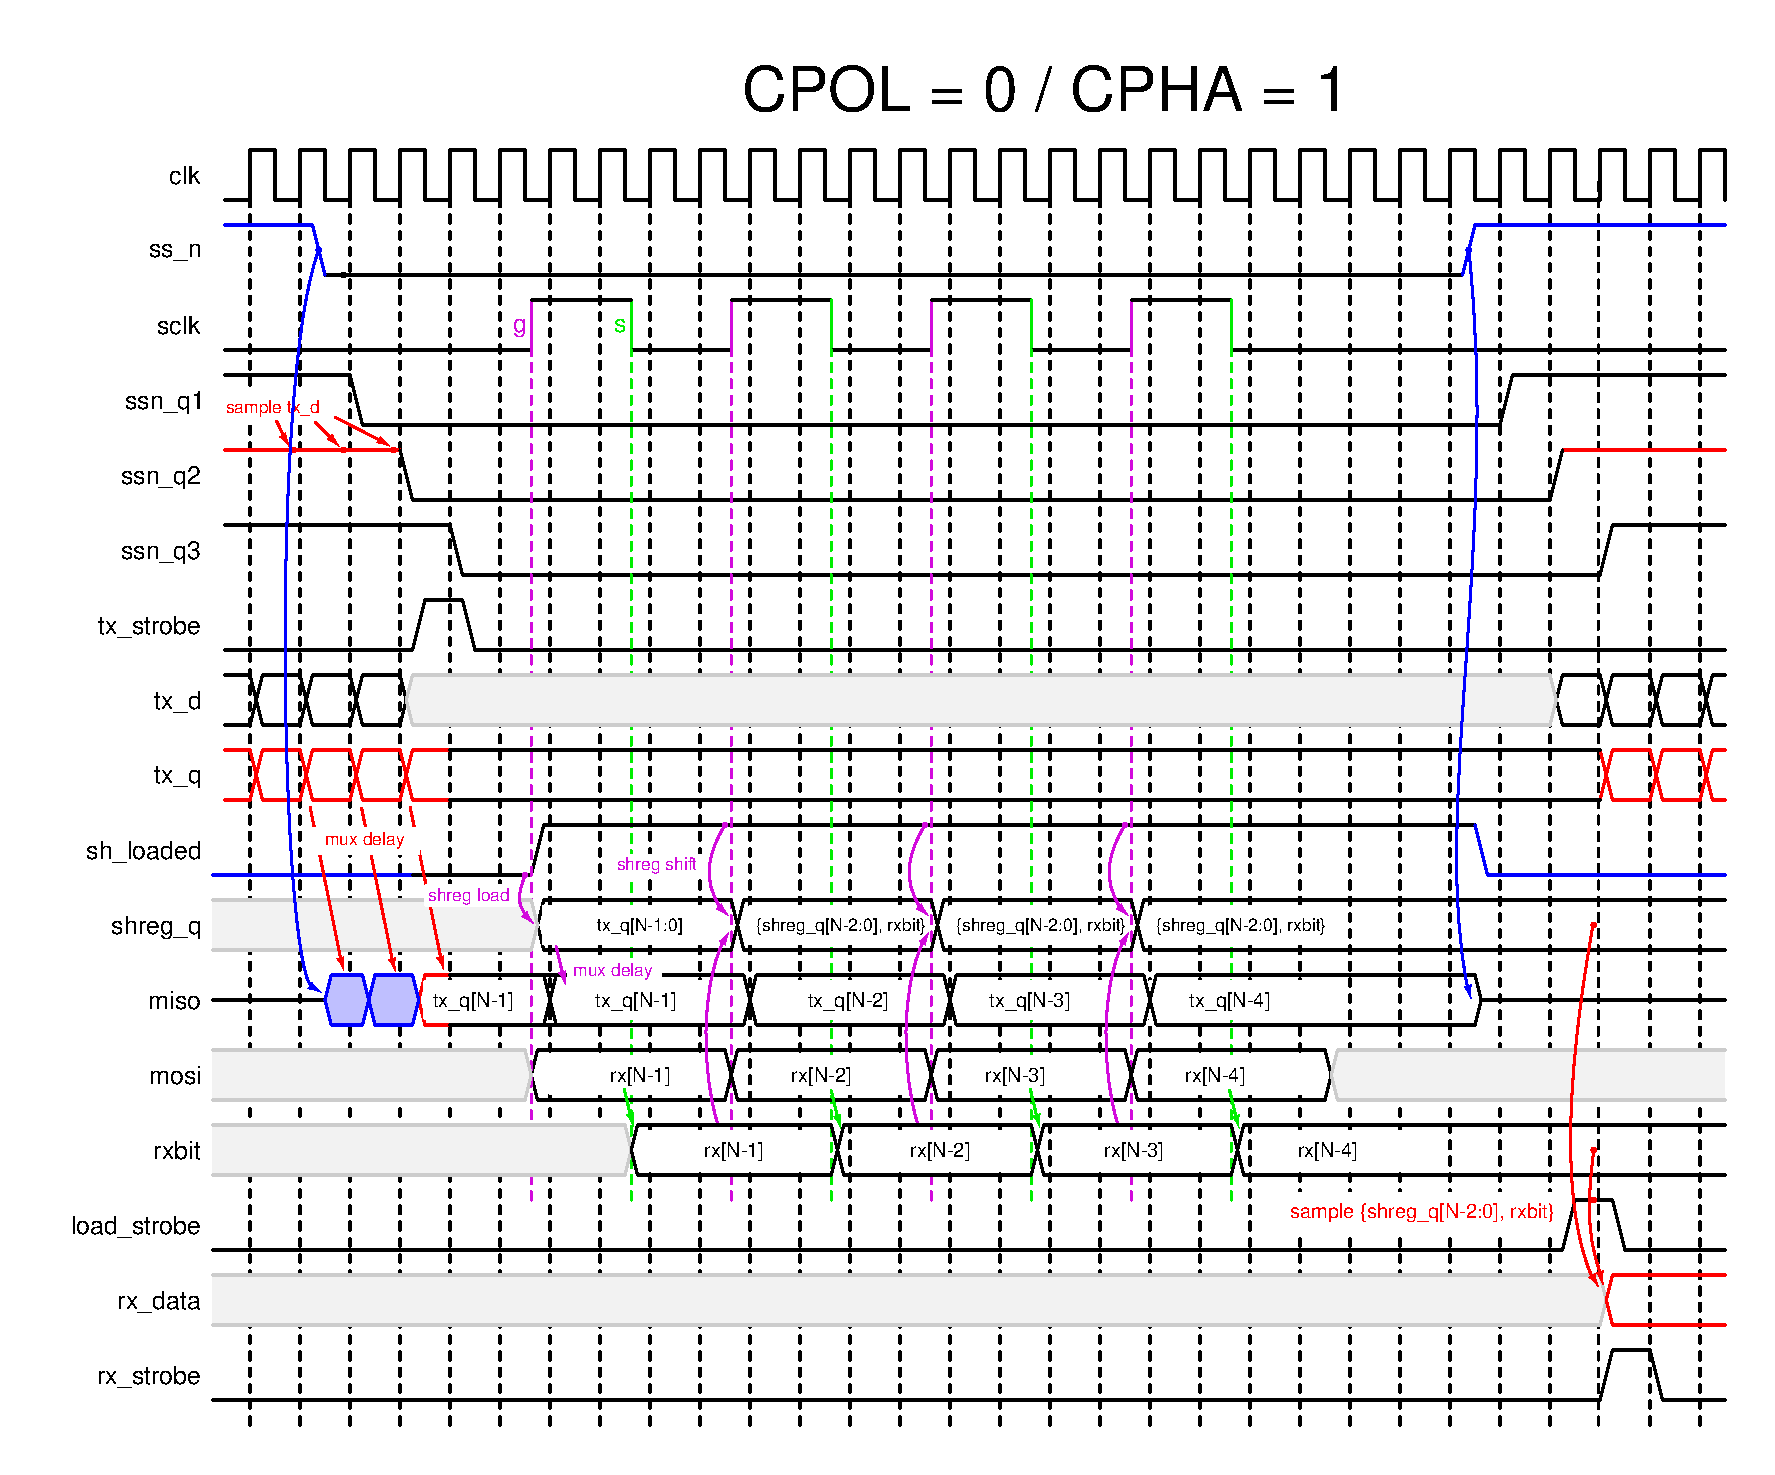
\includegraphics[width=.8\linewidth]{../gfx/spi_timing_cpha1.eps}
    }
    \caption{Manual timing analysis for the SPI slave controller}
    \label{fig:spi_timing}
\end{figure}

\clearpage
\section{UAR(T) Core}\label{apx:uart}

\begin{figure}[h!]
    \centering
    \subfloat[][Datapath]{
        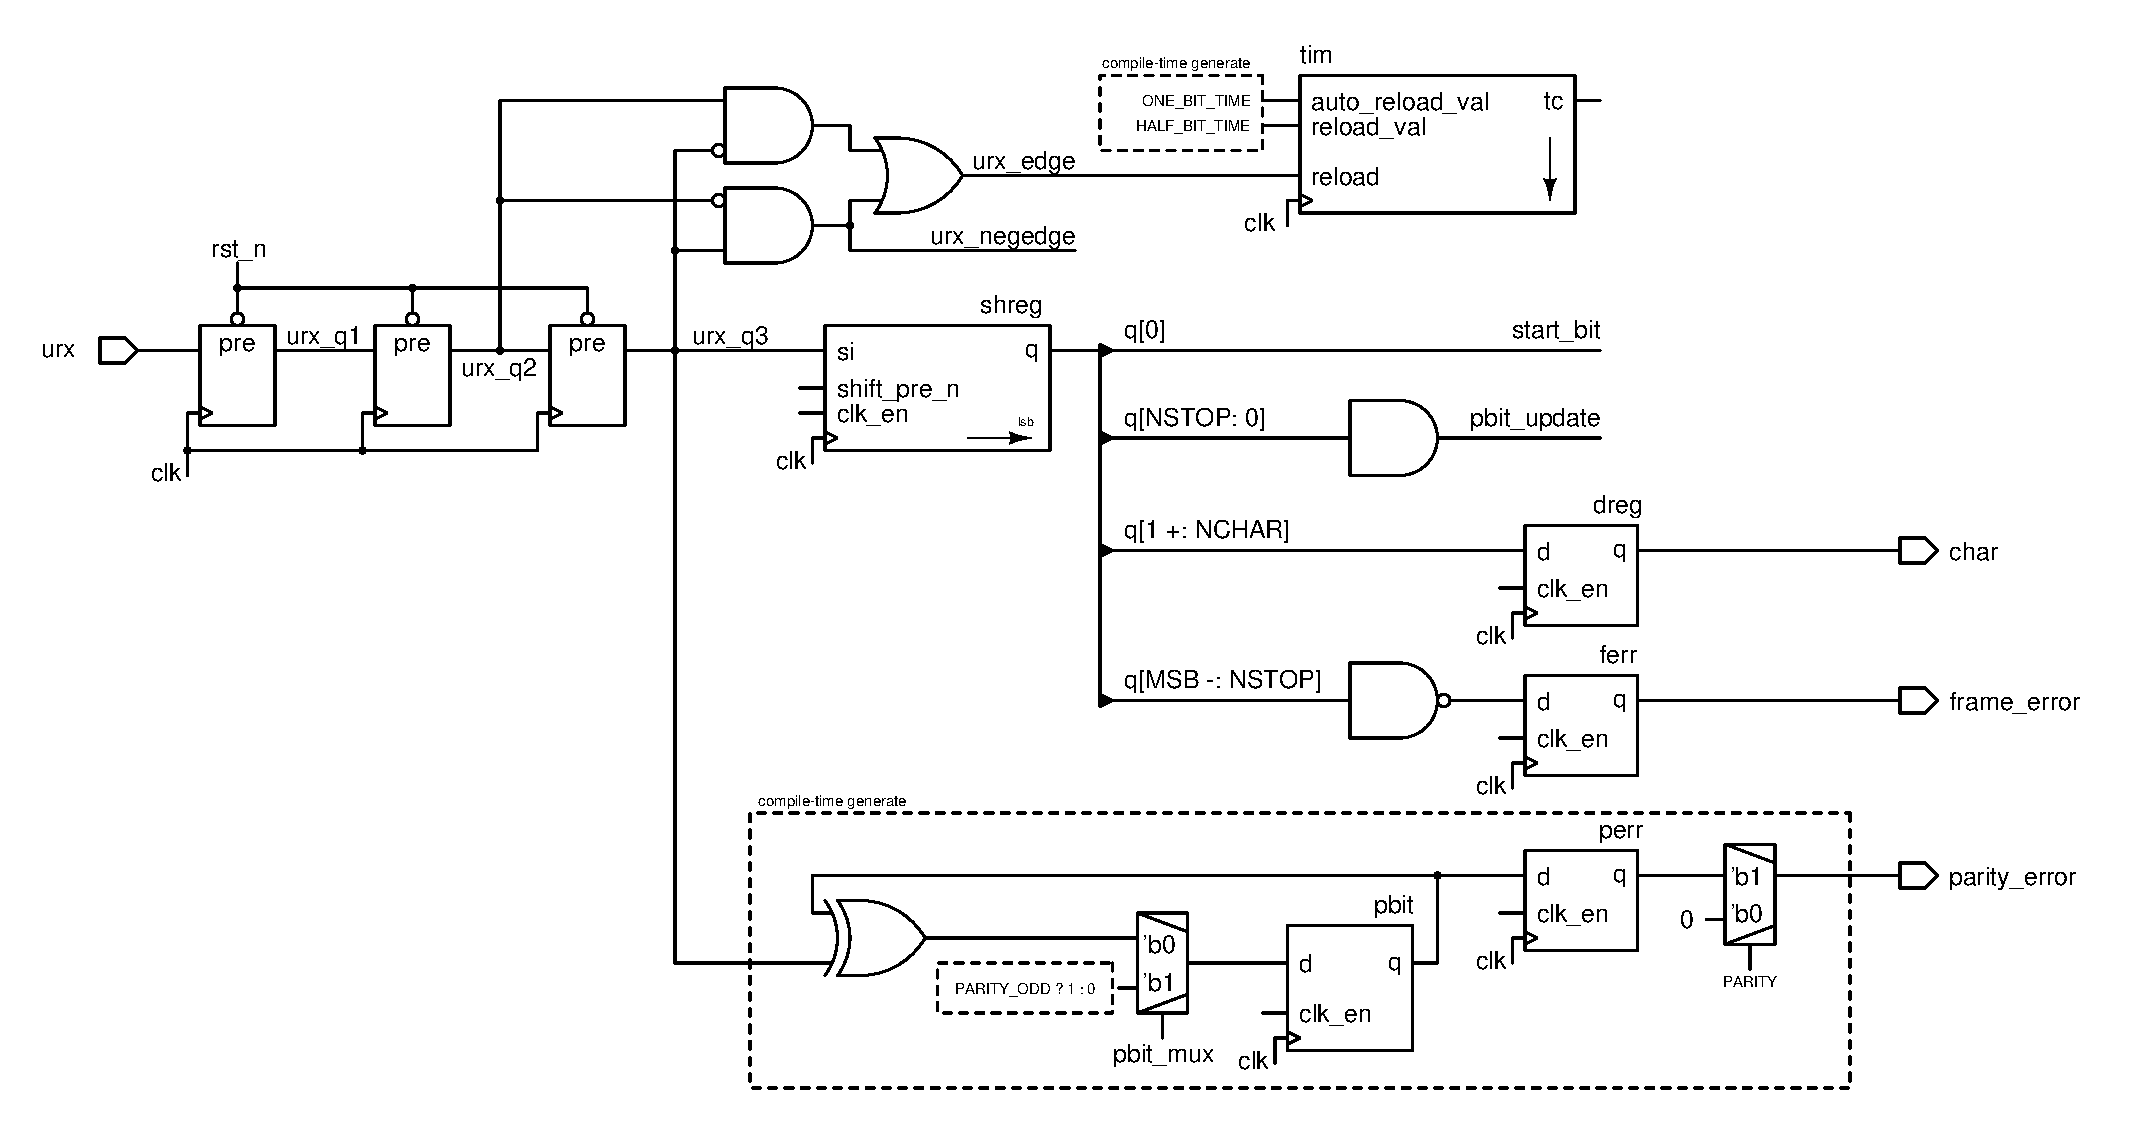
\includegraphics[width=\linewidth]{../gfx/uart_rx_dp.eps}
    }\\
    \subfloat[][ASM detailed chart]{
        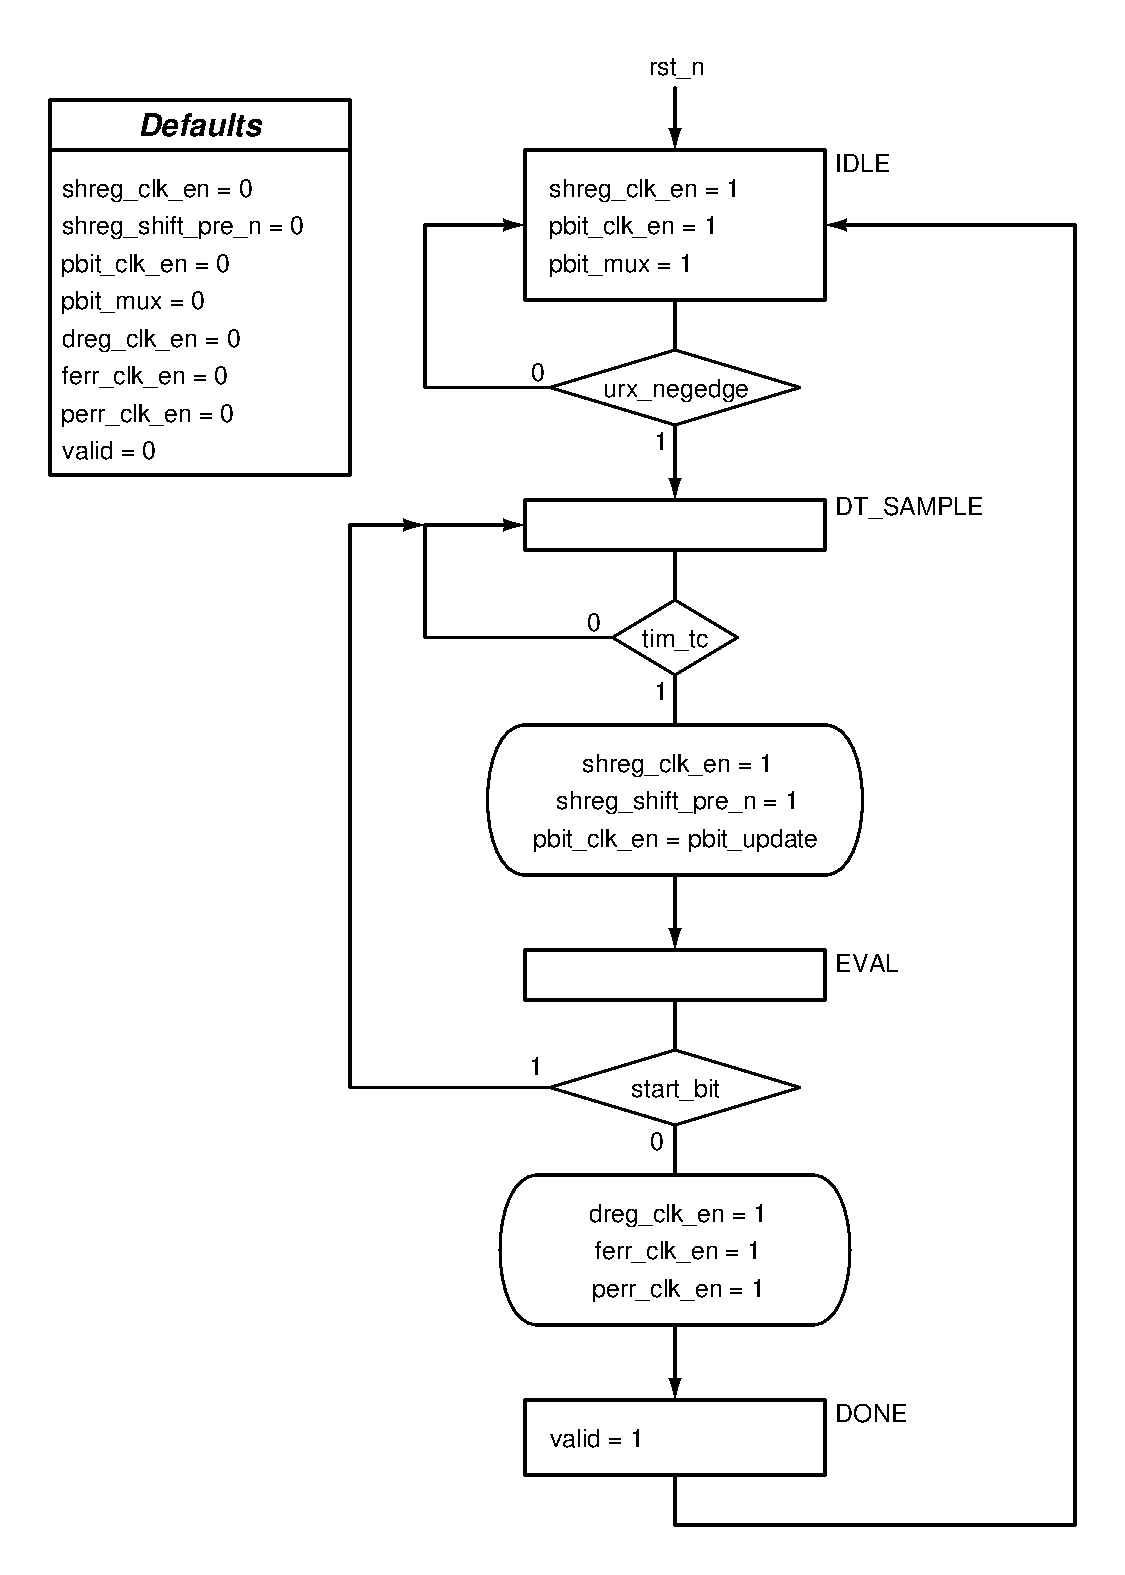
\includegraphics[width=.45\linewidth]{../gfx/uart_rx_asm.eps}
    }
    \caption{UART receiver-only core design}
    \label{fig:uart}
\end{figure}

\end{document}
